 \documentclass[runningheads]{llncs}

% TODO: would you like some consistency work in the notations of transitions (esp. True formula and empty map)

\usepackage{tikz,mathpartir}
\usepackage{mathtools}
\usepackage{amsmath,amssymb,mathabx}
%\usepackage{unicode-math}
\usepackage{tikz}
\usetikzlibrary{external}
\usepackage{hyperref}
\usepackage{nccrules}
\usepackage{comment}
\usepackage{macrospNets}
\usepackage{cancel}
\AtBeginDocument{\renewcommand\setminus{\smallsetminus}}

%\DeclareMathOperator{\dom}{dom}
%\newcommand{\rightarrowdbl}{\rightarrow\mathrel{\mkern-14mu}\rightarrow}

\newcommand{\xrightarrowdbl}[2][]{%
  \xrightarrow[#1]{#2}\mathrel{\mkern-14mu}\rightarrow
}




%\newcommand{\symb}[1]{\makebox{\it #1}}
\newcommand{\dbllbrack}{\{\hspace{-0.88ex}\{}
\newcommand{\dblrbrack}{\}\hspace{-0.87ex}\}}

\newcommand\mpar[1]{{\left(#1\right)}}
\newcommand\mbrk[1]{{\left[#1\right]}}
\newcommand\mbrc[1]{{\left\{#1\right\}}}
\newcommand\mdbrk[1]{\left\ldbrack#1\right\rdbrack}
\newcommand\card[1]{{\left|#1\right|}}
\newcommand\psubst[1]{\mbrc{\!\!\mbrc{#1}\!\!}}
\newcommand\subst[2]{\mbrk{#1\middle/#2}}
\newcommand\midbar{\,\middle|\,}
\newcommand\mset[2]{\mbrc{#1\midbar #2}}

\newcommand\act{\mathrm}
%\newcommand\OTbase[4]{\text{\small\(%
%	\setlength\arraycolsep{2pt}\everymath{\displaystyle}%
%	\renewcommand\arraystretch{1}%
%	\begin{array}{c}%
%	#2,#3,#4 \\\noalign{\color{red}\hrule\vspace{1pt}\hrule}
%	#1
%	\end{array}\)}}
\newcommand\OTbase[4]{\text{\small\(%
	\setlength\arraycolsep{2pt}\everymath{\displaystyle}%
	\renewcommand\arraystretch{1}%
	\begin{array}{c}%
	#2,#3,#4 \\\noalign{\color{red}\hrule}
	#1
	\end{array}\)}}

\newcommand\OThelperdonotuse[2][\top]{\OTtemporary{#1}{\mbrc{#2}}}
\newcommand\OTd[2]{\newcommand\OTtemporary{\OTbase{#1}{\mbrc{#2}}}\OThelperdonotuse}

\newcommand\OT[3]{\OTbase{#1\xrightarrow{\raisebox{-1.5pt}[.8\height][0pt]{\makebox[1.4\width]{\(\scriptstyle #3\)}}}#2}}
\newcommand\OTx[4]{\OT{s_{#1}}{s'_{#1 #2}}{\alpha_{#1 #2}}{\beta_{#3 j}^{j \in J'_{#4}}}{g_{#1 #2}}{\psi_{#1 #2}}}
\newcommand\OTg{\OTx{}{}{}{}}

\theoremstyle{plain}
\newtheorem{thm}{Theorem}
\newtheorem{lem}{Lemma}
\newtheorem{cor}{Corollary}
\newtheorem{prop}{Proposition}

\theoremstyle{definition}
\newtheorem{defi}{Definition}
\newtheorem{exi}{Example}

\newcommand\comment[3]{\colorbox{#1}{#2}\marginpar{#3}}
\newcommand\Rabea{\comment{yellow}}
\newcommand\Ludo{\comment{green}}
\newcommand\Eric{\comment{cyan}}
\newcommand\Quentin{\comment{pink}}

\newcommand\nmm[1]{\(\displaystyle #1\)} % nmm for Nice Math Mode
\newcommand\hyp[1]{\TextOrMath{(H#1)}{\tag{H#1}}}
\newcommand\goal[1]{\TextOrMath{(G#1)}{\tag{G#1}}}
\newcommand\defitem{\item[\bullet]}

\newcommand\setR{\mathbb{R}}
\newcommand\setZ{\mathbb{Z}}
\newcommand\setN{\mathbb{N}}

\newcommand\choice[1]{\left\{\everymath{\displaystyle}%
	\begin{array}{lr}#1\end{array}\right.}
\newcommand\subbox[1]{{\makebox[.5\width]{\(\scriptstyle #1\)}}}
\newcommand\bigsymb[2][\Large]{\text{#1\nmm{#2}}} % DeclareMathDelimiter?
\newcommand\defnotation{\text{ defined as }}
\newcommand\defobject{\DOTSB\;{\coloneq}\;}
\newcommand\nwedge{\DOTSB\;{\wedge}\;} % when you want to force space
\newcommand\qwedge{\DOTSB\quad{\wedge}\quad}
\newcommand\wrel[4][]{#2 \overset{#1}\leq_{#4} #3}
\newcommand\fvars[1]{\mathit{vars}\mpar{#1}}
\newcommand\fguard[1]{\mathit{guard}\mpar{#1}}
\newcommand\fOT[1]{\mathrm{OT}\mpar{#1}}
\newcommand\terms{{\mathcal{T}}}
\newcommand\formulae{{\mathcal{F}}}
\newcommand\actions{{\mathbb{A}}}
\newcommand\rver[3][\!\!]{#2_{#1#3}}
\newcommand\rterms[1][\emptyset]{\rver{\terms}{#1}}
\newcommand\rformulae[1][\emptyset]{\rver{\formulae}{#1}}
\newcommand\ractions[1][\emptyset]{\rver[]{\actions}{#1}}
\newcommand\values{\mathcal{P}}
\newcommand\labels{\mathcal{A}}
\newcommand\reach[1]{\checkmark_{\!\! #1}}

\tikzstyle{every edge} = [draw,-latex,every node/.style={auto}]
\tikzstyle{state} = [draw,circle,minimum size=1cm,inner sep=1mm]
\tikzstyle{initial} = [double,double distance=1mm,minimum size=.95cm,inner sep=.5mm,outer sep=.5mm]
\tikzstyle{init} = [double,double distance=1.5pt,edge label=\(\mbrc{#1}\)]
\tikzstyle{dir} = [out=#1+15,in=#1-15,looseness=10]
%\usepackage{amssymb,amsmath}

\newcommand{\symb}[1]{\makebox{\it #1}} 
\newcommand{\dotcup}{\ensuremath{\mathaccent\cdot\cup}}

\newcommand{\dbllbrack}{\{\hspace{-0.88ex}\{}
\newcommand{\dblrbrack}{\}\hspace{-0.87ex}\}}
\newcommand{\mylangle}{\langle\hspace{-0.58ex}\langle}
\newcommand{\myrangle}{\rangle\hspace{-0.58ex}\rangle}
\newcommand{\subst}[1]{\dbllbrack\!#1\!\dblrbrack}
\newcommand{\Queue}{\symb{Queue}}
\newcommand{\pNet}{P}
\newcommand{\pNetQ}{Q}
\newcommand{\pLTS}{\symb{pLTS}}
\newcommand{\LTS}{\symb{LTS}}
\newcommand{\I}{\mathcal{I}}

\newcommand{\setN}{\mathbb{N}}
\DeclareMathOperator{\futs}{futs}
\DeclareMathOperator{\Sortop}{Sort}
\DeclareMathOperator{\Holes}{Holes}
\DeclareMathOperator{\Leaves}{Leaves}
\DeclareMathOperator{\Label}{Label}
\DeclareMathOperator{\fresh}{fresh}
\newcommand{\Prim}{\symb{Prim}}
\newcommand{\Comp}{\symb{Comp}}
\newcommand{\Component}{\symb{Component}}
\newcommand{\QName}{\symb{QName}}
\DeclareMathOperator{\Enqueue}{Enqueue}
\DeclareMathOperator{\findResult}{findRes}
\DeclareMathOperator{\Observe}{Observe}
\newcommand{\SItf}{\symb{SItf}}
\newcommand{\CItf}{\symb{CItf}}
\newcommand{\Itf}{\symb{Itf}}
\newcommand{\CName}{\symb{CName}}
\DeclareMathOperator{\Name}{Name}
\DeclareMathOperator{\Interfaces}{Interfaces}
\DeclareMathOperator{\GetItf}{Get}
\DeclareMathOperator{\UniqueItfNames}{UniqueItfNames}
\newcommand{\SM}{\symb{SM}}
\newcommand{\MC}{\symb{MC}}
\newcommand{\CM}{\symb{CM}}
\newcommand{\Let}{\text{let}}
\newcommand{\In}{\text{in}}
\DeclareMathOperator{\MethLabel}{MethLabel}
\DeclareMathOperator{\Symm}{Symm}
\DeclareMathOperator{\dom}{dom}
\DeclareMathOperator{\codom}{codom}
\DeclareMathOperator{\Gmax}{Gmax}
\DeclareMathOperator{\Index}{Index}
\newcommand{\Target}{\symb{Target}}
\DeclareMathOperator{\Id}{Id}

\newcommand{\Act}{\symb{Act}} 
\newcommand{\fv}{\symb{fv}}
\newcommand{\iv}{\symb{iv}}
\newcommand{\vars}{\symb{vars}}
\newcommand{\BC}[2]{\symb{BC}_{#1}(#2)}
\newcommand{\PNfamily}[2]{\overleftrightarrow{\mylangle#2,#1\myrangle}}
\let\oldmapsto\mapsto
\renewcommand{\mapsto}{\text{\scriptsize{$\oldmapsto$}}}
\newcommand{\set}[1]{\overline{#1}}

\newcommand{\Sort}{\symb{Sort}}



\DeclareMathOperator{\card}{card}
\DeclareMathOperator{\Flat}{Flat}
\renewcommand{\P}{\mathcal P}
\newcommand{\OTarrow}[1]{\textcolor{red}{\,\xrightarrow{\textcolor{black}{#1}}\,}}
\newcommand{\OTWeakarrow}[1]{\textcolor{red}{\,\xRightarrow{\textcolor{black}{#1}}\,}}

\def\AlgT{\mathcal{T}}
\def\AlgE{\mathcal{E}}
\def\AlgA{\mathcal{A}}
\def\AlgAS{\mathcal{A}_S}
\def\AlgB{\mathcal{B}}
\def\AlgI{\mathcal{I}}

\newcommand{\CreateISet}[2]{[#1]_{#2}}

\makeatletter
\def \dotover {\textcolor{red}{\leavevmode\cleaders\hb@xt@ .22em{\hss 
$\cdot$\hss}\hfill\kern\z@}}
\def \reddottedrule #1#2{\hbox {\advance \hsize by -0.5em
%\sbox0{$\genfrac{}{}{0pt}{0}{#1}{#2}$} \phantom{\copy0} %
 {\ooalign{\vphantom{$\genfrac{}{}{0pt}{0}{#1}{#2}$}\cr\dotover\cr$\genfrac{}{}{0pt}{0}{#1}{#2}$\cr}}}}

 \def \dottedrule #1#2 {
  {\sbox0{$\genfrac{}{}{0pt}{0}{#1}{#2}$}%
    \vphantom{\copy0}%
    \ooalign{%
      \hidewidth
      $\vcenter{\moveright\nulldelimiterspace
        \hbox to\wd0{%
         \xleaders\hbox{\kern.5pt\vrule height 0.4pt width 1.5pt\kern.5pt}\hfill
          \kern-1.5pt
        }%
      }$
      \hidewidth\cr
    \box0\cr}}
}

\let \defaultfraction \mpr@@fraction
\makeatother


% Macros for the SOS rules and proof trees:
%\newcommand\openrule[2]{\redinfer{#1}{#2}}
\newcommand\openrule[2]{\mprset{myfraction=\reddottedrule}\inferrule{#1}{#2}}
%\newcommand\openrule[2]{\inferrule*{#1}{#2}}
%\newcommand\ostate[1]{\triangleleft{\;#1\;}\triangleright}
\newcommand\ostate[1]{\triangleleft{#1}\triangleright}
\newcommand{\sm}[1]{\mbox{\boldmath\small #1}}

\newcommand{\Pred}{\symb{Pred}}
\newcommand{\Post}{\symb{Post}}
\newcommand{\SV}[3]{#1\to #2 [#3]}
\newcommand{\Predsv}{\Pred_{\symb{sv}}}
\newcommand{\TrUn}{\textbf{Tr1}}
\newcommand{\TrDeux}{\textbf{Tr2}}
\newcommand{\vis}[1]{(#1)^*}

%%% weak automaton

\def\WT{\mathcal{WT}}
\def\WOT{\symb{WOT}}

\newcommand{\True}{\symb{True}}


\begin{document}
%
\title{Refinements for open automata}



%
%\titlerunning{Abbreviated paper title}
% If the paper title is too long for the running head, you can set
% an abbreviated paper title here
%
\author{
Rabéa Ameur-Boulifa\inst{1}\orcidID{0000-0002-2471-8012} \and
Quentin Corradi\inst{2}\orcidID{0000-0003-4218-3987} \and
Ludovic Henrio \inst{2}\orcidID{0000-0001-7137-3523} \and
Eric Madelaine \inst{3}\orcidID{0000-0002-5552-5993}}
%
\authorrunning{Rab\'ea Ameur-Boulifa et al.}
% First names are abbreviated in the running head.
% If there are more than two authors, 'et al.' is used.
%
\institute{LTCI, T\'el\'ecom Paris, Institut Polytechnique de Paris, France
\email{first.last@telecom-paris.fr}\\
\and
Universit\'e Lyon, EnsL, UCBL, CNRS, Inria,  LIP, France\\
\email{first.last@ens-lyon.fr}
 \and
INRIA Sophia Antipolis M\'edit\'erann\'ee, UCA,  France
\email{first.last@inria.fr}}
%
\maketitle              % typeset the header of the contribution
%
\begin{abstract}
%\TODO{ The abstract should briefly summarize the contents of the paper in 150--250 words.}

Establishing equivalence and refinement relations between programs is an important mean for 
verifying their correctness. By establishing that the
behaviours of a modified program simulate those of the source one, bisimulation relations formalise the desired relation between a specification and an implementation, 
 two equivalent implementations, or a program and its optimised implementation.
This article discusses a notion of refinement between \emph{open automata}, which are symbolic
behavioural models for communicating systems. 
Open automata may have \emph{holes} modelling elements of their
context, and can be composed by instantiation of the holes. This allows for a compositional approach for
verification of their behaviour.

We define several variants of refinement relations between systems including either equal or different sets of holes, and 
show under which conditions these refinements are preserved by composition of open automata. 


\keywords{Labelled transition systems  \and Refinement \and Composition.}
\end{abstract}
%
%
%
\section{Introduction}


\TODO{TODO list}


* \st{example a terminer}

* choisir terminologie: refinement or simulation

* open automata  / Open Automata -> only use open automata or OA.

* positioning

* \st{format according to conf: lncs FACS or SEFM}

* global rewriting (partly done)





Automata are convenient for specifying and verifying systems, but most automata definitions allow only the specifications of finite closed systems. Indeed those systems are the ones we can verify efficiently, but programming often consists in writing open systems that should be interfaced with others, and with potentially unbound behaviours (at least statically). We investigate in our works the possibility to define open symbolic systems, verify some of their properties, and use them to compose in a structured way more complex systems.


\RAB{The refinement concept plays  an important role in software engineering. In addition to helping to cope with the complexity, refinement provides a foundation for ensuring  system (software) correctness. The correctness of a system can
be established by proving, that a system refines its specification.}
%Refinement relations verify that an implementation satisfies some properties with respect to a specification. 
Refinement entails that one system  can be considered as a more precise version of the specification, featuring all the specified behaviours with more concrete details. From  formal point of view,  refinement can be defined as a mathematical relations between a specification and its implementation. It is usually defined as trace inclusion or simulation  \cite{Milner:1980,Kouchnarenko:2007}. Each  offers specific guarantees on the  behavioural properties of the specification, and it ensures that all behaviours of the specification must belong to the behaviours of the implementation. This definition, which is based on systems whose behaviour is fully defined, is not well-suited for open systems,  as it requires to reason also about unspecified behaviours.



Open automata (that we abbreviate OA) were defined as a way to provide a semantics for open parameterized hierarchical LTSs used in verification tools and called \emph{pNets}.
An OA \cite{henrio:01299562} is a classical automaton with variables and holes. Variables make automata symbolic and allow them to encode infinite state systems. Holes enable the composition of automata: an automaton with a hole is an operator that takes another automaton as parameter and reacts to the actions it emits; the composed automaton is a more precise automaton where the behaviour of one ``process parameter'' % \TODO{est-ce qu'on n'ecrirait pas ici "process parameter" pour les distinguer des variables standard ?}
% LUDO: DONE
 of the main automaton has been provided.

In previous works \cite{AMHEEMA:2023,wang:03126313} a bisimulation relation was defined for OA and open parameterized hierarchical LTSs. It has already good properties relatively to bisimulation, but refinement relations were not studied. In this article we go further to  define a theory of refinement to OA. The refinement relation we introduce in the paper  is based on the notion of   simulation,  in a similar way to that defined in classical automata theory \cite{Milner:1989,Bellegarde:2000}.  And with the common behaviour-preserving  property:  all the behaviour of the abstract specification must be followed by its (complex) implementation but additional behaviours may exist. However we also ensure that a whole scenario, made of several steps, of the specification can also be simulated by the refined system, which is slightly richer than the traditional simulation relation and which allows us to obtain a compositionality result.

%This article first introduces OA that were defined in  \cite{henrio:01299562}. %,  but compared to previous works, we and additionally defines the composition of OA.
Our contribution in this paper is the definition a refinement relation for OA that has the following characteristics:
\begin{itemize}
\item Classical simulation characterisation but also an additional criteria ensuring that refinement does not introduce deadlocks when following a trace from the simulated automaton.
\item Good properties relatively to composition: we prove here that filling the same hole  with the same automaton preserves the refinement relation.
\item Ability to take into account both composition and transitivity: this is a challenge because composition changes the set of holes of the OA and refinement takes into account the actions of the holes.
\end{itemize}
The refinement relation is introduced in two steps. First we define a refinement that relates two automata with the same holes, which allows us to focus on the automaton aspect. Second we introduce a relation that relates two automata with different sets of holes, which allows us to take into account the open nature of OA, and to deal with composition. Properties of the refinement are stated and proven on the second, more general version of the relation, they are thus also valid for the first simpler refinement relation.

The following of this article is organised as follows. 
Section~\ref{sec:background} recalls the definition of open automata and defines their composition. 
We  then  define a refinement relation for OA, first only considering two automata with the same set of holes in Section~\ref{sec:refinement} and generalize it to automata with a different set of holes in Section~\ref{sec:holes}.  Section~\ref{sec:prop} is dedicated to formalize and prove basic properties of refinement in ; here we prove that refinement is a preorder and has good composition property. 
In Section~\ref{sec:sota} we review related works, and Section~\ref{sec:ccl} concludes the paper.


\section{Open Automata and their Composition}\label{sec:background}

This section presents our notations and the principles of automata. Except for minor changes in the notations, compared to previous works~\cite{fhbisim} the only new contribution is the definition of a composition operator for OA.
%
%Notations will be defined with the operator \(\defnotation\) and names are given with the operator \(\defobject\) as follows:
%\begin{align*}
%	\mathit{notation\_with\_variables} & \defnotation \mathit{notated\_object\_using\_the\_variables} \\
%	\mathit{name} & \defobject \mathit{fully\_defined\_mathematical\_object}
%\end{align*}

%Throughout this paper, tuples will be noted differently depending on what they represent.
%This helps distinguishing the manipulated objects.
%Every such notation will be introduced in the definition of the object.


\subsection{Preliminaries and notations}
Families of values, or equivalently maps will be noted \(x_i^{i \in I}\), \(\mset{i \mapsto x_i}{i \in I}\), or \(\mset{i \gets x_i}{i \in I}\), depending on what is more convenient (e.g. $i \gets x_i$ is used for maps that are used as substitution). Statements like  $\exists c_j^{j \in J}$ defines both $J$ and the mapping ${j \mapsto c_j}$.
%For instance \(\mpar{ax}^{x \in \setR}\) represents a scaling function, \(c^{i \in I}\) is a constant function over \(I\).
%They will be used depending on what is more convenient.
%For instance \(\mbrc{\alpha \mapsto 1, \beta \mapsto 2, \gamma \mapsto 3}\) has no simple generating expression and is better represented with the finite version of first notation.
The disjoint union on sets is noted \(\uplus\).
%\footnote{Depending on the context, \(\uplus\) notation either supposes that the sets are disjoint or constraints joined sets to be disjoints if several choices are possible}.
Disjoint union is also used on maps.
There are several ways of ensuring a union is disjoint, we will indifferently either suppose sets are disjoint or rename conflicting objects (useful for variables).
%The disjoint union of two maps \(\varphi: I \to X\) and \(\psi: J \to Y\) with \(I \cap J = \emptyset\) is noted \(\varphi \uplus \psi\) and has the following signature \(I \uplus J \to X \cup Y\).
In a formula, a quantifier followed by a finite set will be used as a shorthand for the quantification on every variable in the set:
\(\forall \mbrc{a_1, \dots, a_n}, \exists \mbrc{b_1, \dots, b_m}, P\) means \(\forall a_1, \dots, \forall a_n, \exists b_1, \dots, \exists b_m, P\).

%\begin{definition}[Expression algebra, Action algebra, Formulas, Terms]
Our expression algebra \(E\) is the disjoint union  of  terms,  actions, and  formulas
\( E=\terms \uplus \actions \uplus \formulas\) .
\(\terms\) and \(\actions\) are term algebras.
The formulas \(\formulas\) contain at least first order formulas and equality\footnote{Equality does not need to be only syntactic.} over \(\terms\) and \(\actions\). 
%\end{definition}
For \(e \in E\),
 \(\fvars{e}\) is the set of variables in  $e$ that are not bound by a binder. 
An expression is closed if \(\fvars{e}=\emptyset\).
The set \(\values\) denotes values which is a subset of closed terms. \(\rformulas[V]\) is the set of formulas $f$ that only uses variables in $V$, i.e. the formulas such that  \(\fvars{f}\subseteq V\).
%The substitution in \(e \in E\) of \(x \in \fvars{e}\) by \(t \in \terms\), is denoted \(e\subst{t}{x}\), and its generalisation to t
The parallel substitution of variables in \(V\) by a map \(\psi: V \to \terms\) is denoted \(e\psubst{\psi}\).


 We suppose given a decidable satisfiability relation on closed formulas, denoted \({\vdash} f\).
% In practice one of our objective is to be able to use a SMT solver to reason automatically on the properties of open automata, in this case
%\(\vdash\) can hence be interpreted as an indicator of what is given to the SMT; it separates the external logic and the logic on \(\formulas\).
We will use two variants of the satisfiability relation:
\begin{itemize}
\item The satisfiability of a formula \(f \in \formulas\) under some valuation \(\sigma: V \to \values\) is defined as follows:
\( \sigma \vdash f \iff \vdash \exists \fvars{f\psubst{\sigma}}, f\psubst{\sigma} \)
\item The satisfiability of a formula \(f \in \formulas\) with some variable set \(V\) as context is defined as follows:
\( V \vdash f \iff  \vdash \forall V, \exists\mpar{\fvars{f} \setminus V}, f \)
\end{itemize}

%For instance a formula with quantifiers on variables might not be provable even if it is true for all values of these variables.

\subsection{Open Automata (OA)}\label{sec:def}
 OA  are labelled transition systems with variables  that can be used to compose other automata: they are made of transitions that are dependent on the actions of ``holes'', a composition operation consists in filling a hole with another automaton to obtain a more complex automaton. The variables makes the OA symbolic, and the holes allow for a partial definition of the behaviour.

\begin{definition}[Open transition, Open automaton]
An \emph{open automaton} is a tuple \(\OAg\) with \(S\) a set of states, \(s_0 \in S\) the initial state, \(V\) the finite set of variable names, \(\sigma_0: V \to \values\) the initial valuation of variables, \(J\) the set of hole names and \(T\) the set of open transitions. 

An \emph{open transition} is a tuple \nmm{\OTg} with \(s, s' \in S\) the source and target states, \(\alpha \in \actions\) the produced action, \(J' \subseteq J\) the holes involved in the transition, \(\beta_j \in \actions\) the actions of the holes, \(g \in \formulas\) the guard and \(\psi: V \to \terms\) the variable assignments.
To be well-formed, an open transition should use only variables of the automaton and variables appearing in the involved actions, formally: 
\begin{align*}
\fvars{g}&\subseteq \fvars{\alpha}\cup \bigcup_{j \in J'} \fvars{\beta_j} \cup V \\ \forall v\in V.\, \fvars{\psi(v)}&\subseteq \fvars{\alpha}\cup \bigcup_{j \in J'} \fvars{\beta_j} \cup V
\end{align*}
\end{definition}



We use two operators to access pieces of information of the OA.

%\TODO{useful or not?}
\begin{definition}[Out-transition, Transition variables]
Let \(V\) be the variable names of the considered automaton, \(T\) its transitions and \(r\) one of its states.
\(\fOT[T]{r} \subset T\) are called the out-transitions of the state \(r\).
%\(\fIT[T]{r} \subset T\) are called the in-transitions of the state \(r\).
When the transition set is clear from the context, it will be omitted.
The local variables of a transition \(\fvars{t}\) are all variables appearing in transition \(t\) except the variables of the automaton.
%\begin{align*}
% %&
%%	\fIT[T]{r} & = \mset{\OTg \in T}{s' = r} \\
%\end{align*}
%\vspace{-1cm}
\begin{mathpar}
%	\fguard{\OTg} \!=\! g \qquad
	\fOT[T]{r}  = \mset{\OTg \in T}{s = r}

	\fvars{\OTg} \!=\! \mpar{\fvars{\alpha}  \cup \bigcup_{j \in J'} \!\fvars{\beta_j} } \setminus V
\end{mathpar}
\end{definition}

A pair consisting of a state and a valuation is called a \emph{configuration}.
%
%The following terminology will be used to reason on open automata
%\begin{definition}[Configuration, instantiated transition]
%An \emph{instantiated transition} of an automaton \(\OAg\) is a transition  \(t\psi\) where $t\in T$ and $\psi$ is a  well-formed substitution with $\dom(\psi)=vars(t)$. %\setminus V$.
%\end{definition}



\begin{example}[\texttt{prod-cons}]\label{Example:fifo-system} As a running example, we consider a classical producer-consumer pair  interacting through FIFO buffer, named \texttt{prod-cons}.  Fig. \ref{Fig:Architect} reflects the overall structure of the system involving a producer process, a consumer process and an orchestrator that coordinates  their activities. 

\begin{figure}[!ht]
 \centering
   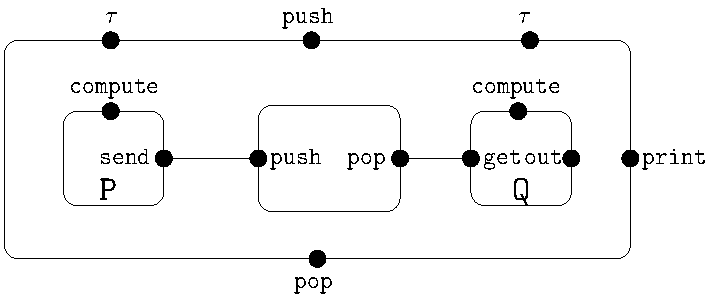
\includegraphics[width=.70\textwidth]{Figures/Architecture.pdf}
   \caption{Structure of the example. Each box corresponds to a process whose ports are the actions it can perform. The  actions observable by the environment are $\texttt{push}$, which indicates the enqueuing of an element, $\texttt{pop}$ which indicates the dequeuing, and $\texttt{print}$ which indicates the production of results. \label{Fig:Architect}} 
\end{figure}

The example uses several kinds of data. Variable $\texttt{m}$ holds a message, message types do not need a concrete definition here. We additionally use arrays of messages with a syntax of the form $\texttt{M[l]}$ for array accesses; $\texttt{M}$ is an array of $\texttt{N}$ elements, from $0$ to $\texttt{N}-1$. Finally we use addition and modulo operation ($\%$) on integers.

The OA  modelling the behaviour of such a system  using an  unbounded circular/ring buffer is depicted in Fig. \ref{Fig:RefineOA}.  The automaton has a single state with  two holes: $\texttt{P}$ and  $\texttt{Q}$ that are the two interacting processes.  $\texttt{l}$   indicates the next available position for  enqueuing an element  and  $\texttt{f}$ is the position that contains the next element to be dequeued. %\footnote{The  arrow  without any state of origin is a graphical convention to indicate that the pointers are initialized at the beginning}. 
The buffer reacts to a push from $\texttt{P}$ and enqueues it. Similarly, whenever   $\texttt{Q}$ pops an element, it dequeues it. Additionally, whenever $\texttt{Q}$ produces an item, it is exposed as an external observable  $\texttt{print}$ action. 
When any process do its internal computation, it is exposed externally as unobservable action $\tau$. 
\begin{figure}[!tb]
 \centering
   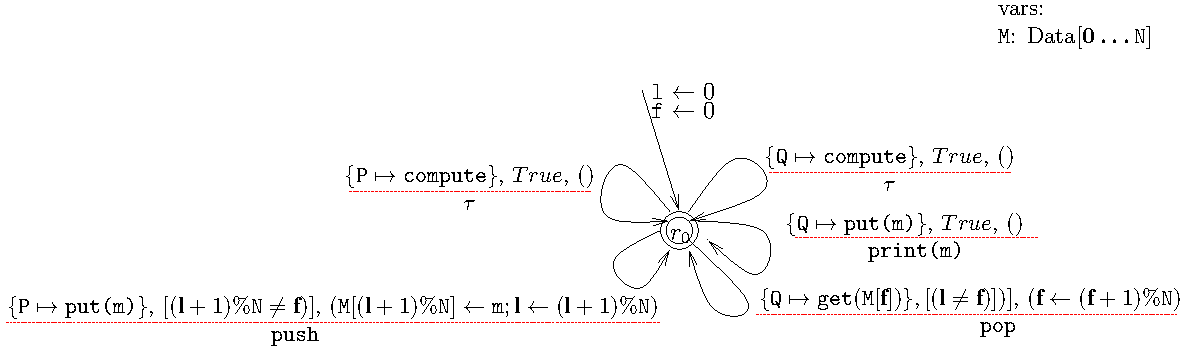
\includegraphics[width=.99\textwidth]{Figures/FIFORing.pdf}
   \caption{Open automaton for the \texttt{prod-cons} system using FIFO circular buffer.
    \label{Fig:RefineOA}} 
\end{figure}
\qed
\end{example}





\paragraph{Open automaton composition.}

OA are partially specified automata, the partiality arises  from the holes.
A hole can be seen as a port in which we can plug an OA.
The plugging operation is called composition.
The composition of OA was already implicitly defined by the means of composition on pNets in previous work \cite{henrio:01299562} but never  formalised on OA.\footnote{The definition of composition below is a direct translation of what happens with pNets composition \cite{henrio:01299562} without  introducing pNets.}





\begin{definition}[Composition of open automata] \label{Def:CompOA}
% TODO: this definition is a bit strange, why is Ac in the hole of Ap but the hole is in Ac and the notation is reversed?
Let  \(A_c = \OAg[c]\) be a context OA and $k$ one of its holes, \(k \in J_c\). Let \(A_p = \OAg[p]\) be an OA,  the composition $A_c\subst{A_p}{k}$ is defined as follows:
\[A_c\subst{A_p}{k} ::=  \OA{S_c \times S_p}{\mpar{s_{0c}, s_{0p}}}{V_c \uplus V_p}{\sigma_{0c} \uplus \sigma_{0p}}{J_p \uplus J_c \setminus \mbrc{k}}{T} \] \text{with }
\begin{align*}
T\!=& \mset{\OT{\mpar{s_c, s_p}}{\mpar{s'_c, s'_p}}{\alpha_c}{\beta_j^{j \in J'_p \uplus J'_c}\!}{g_c \wedge g_p \wedge \alpha_p = \beta_k}{\psi_c \uplus \psi_p}}{ \OT{s_c}{s'_c}{\alpha_c}{\beta_j^{j \in J'_c \uplus \mbrc{k} }\!}{g_c}{\psi_c} \in\! T_c, \OTx{p}{}{}{p} \in\! T_p} \\
	& \cup \mset{\OT{\mpar{s_c, s_p}}{\mpar{s'_c, s_p}}{\alpha_c}{\beta_j^{j \in J'_c}}{g_c}{\psi_c}}{\OTx{c}{}{}{c} \in T_c, k \notin J'_c, s_p \in S_p}
\end{align*}
\end{definition}

The first OA decides when the second can evolve by involving its hole in a transition: the action emitted when \(A_p\) makes a transition is synchronised with the action of the hole \(k\) in transitions of \(A_c\).



\begin{example} \label{Example:prodandcons} Fig. \ref{Fig:procandcons} shows a producer automaton  and a consumer  automaton that can be used  to fill the holes $\texttt{P}$ and $\texttt{Q}$ of \texttt{prod-cons} defined in Example~\ref{Example:fifo-system}.
 \begin{figure}[!ht]
 \centering
   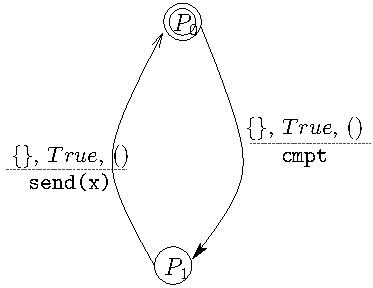
\includegraphics[width=.35\textwidth]{Figures/P-proc.pdf}\hfill 
   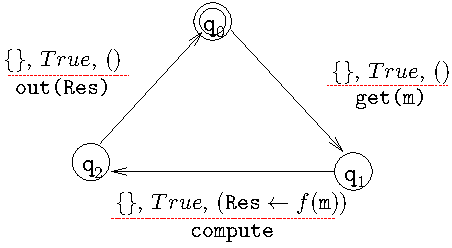
\includegraphics[width=.45\textwidth]{Figures/Q-proc.pdf}
   \caption{(Left) A \texttt{producer}.  It produces one item at a time and pushes it.  (Right)  A \texttt{consumer}. It pops an item, does some work and pushes the result. \label{Fig:procandcons}}
\end{figure}



The OA on Fig. \ref{Fig:ComposeOA} is the composition of the system in Fig.~\ref{Fig:RefineOA} and the producer in Fig. \ref{Fig:procandcons} (left). The composition consists of two states (the product of the states of both automata). The transitions from one state to another come from  the synchronisation  of the transitions of the encompassing automaton with those of the producer filling the hole $\texttt{P}$. Transitions involving \texttt{Q} remain unchanged. \qed


\begin{figure}[!ht]
 \centering
   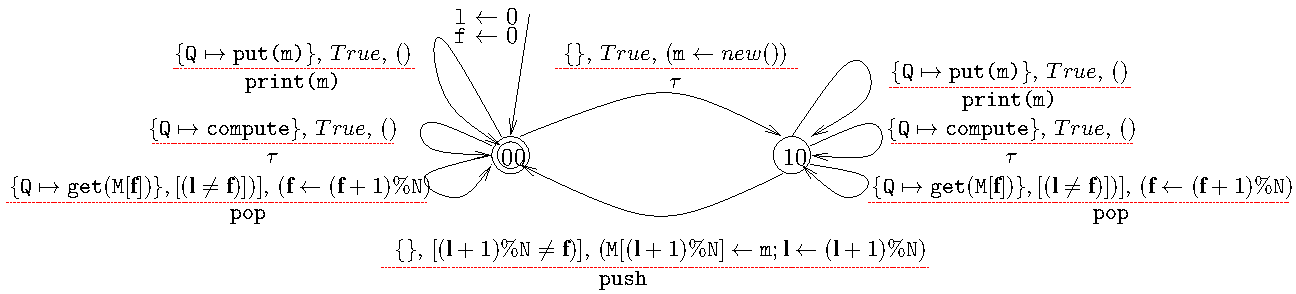
\includegraphics[width=.99\textwidth]{Figures/compos-FIFO-Pro.pdf}
   \caption{Open automaton for \texttt{prod-cons}[\texttt{P}/\texttt{producer}]. 
   \label{Fig:ComposeOA}} 
\end{figure}
\end{example}



\subsection{Relations between open automata}
Establishing semantic equivalences and refinement relations between different OA requires  to compare their states. For this purpose, we suppose that the variables of the two OA are disjoint (a renaming of variables may have to be applied before comparing OA states).
\begin{definition}[Relation on open automata configurations] Suppose $V_1$ and $V_2$ are disjoint.
A relation on configurations of two OA \(\OAg[1]\) and \(\OAg[2]\) is a function \(R: S_1 \times S_2 \to \rformulas[V_1 \uplus V_2]\).
\end{definition}
%\TODO{C'est etrange, la formulation "the variables they refer to", comme il n'y a plus de variables d'etat... +1}
The idea is that two states are related depending on the satisfiability of the expression relying their variables i.e., if the variables of the OA verify a certain formula. 
In other words, to each pair of states is attached a boolean formula that may refer to the  variables of each of the two OA, stating whether the two states are related or not.
Additionally, we may check that initial states of the automata are related by checking that: \(\sigma_{01} \uplus \sigma_{02} \vdash R\mpar{s_{01}, s_{02}}\).

%\TODO{I do not think we reason on configurations for the moment, if we want to, we should introduce this:}
%Two configurations \(\mpar{s_1, \sigma_1} \in S_1 \times\mpar{V_1 \to \values}, \mpar{s_2, \sigma_2} \in S_2 \times \mpar{V_2 \to \values}\) are related iff \(\sigma_1 \uplus \sigma_2 \vdash R\mpar{s_1, s_2}\).

\subsection{A bisimulation for open automata}

Bisimulation between OA was defined in~\cite{fhbisim}.  We show below the principles of this bisimulation. We first recall the usual definition of bisimulation.
Bisimulation can  be defined as follows for standard transition systems: 

\begin{definition}[Classical Bisimulation]
  A bisimulation is a relation $\mathcal{R}$ such that $s~\mathcal{R}~t$:\\
  \begin{minipage}[c]{.6\textwidth}
    \[
      \forall l~s',~ {s}\xrightarrow{l}{s'}
      \implies
      \exists t'.~ s' ~\mathcal{R}~ t'
      \land {t}\xrightarrow{l}{t'}
    \]
    \begin{center}
      and conversely
    \end{center}
    \vspace{-1ex}
    \[
      \forall l~t',~ {t}\xrightarrow{l}{t'}
      \implies
      \exists s'.~ s' ~\mathcal{R}~ t'
      \land {s}\xrightarrow{l}{s'}
    \]
    \vspace{.5ex}
  \end{minipage}
  i.e. \qquad
  \begin{minipage}[c]{.35\textwidth}
    \begin{tikzpicture}
      \node (s) at (-1,1) {$s$};
      \node (R) at (0,1) {$~\mathcal{R}$};
      \node (t) at (1,1) {$t$};
      \node (sp) at (-1,0) {$s^\prime$}
      edge [<-] node[auto] {$l$} (s);
      \node (Rp) at (0,0) {$\mathcal{R}$};
      \node (tp) at (1,0) {$t^\prime$}
      edge [<-] node[auto,swap] {$l$} (t);
    \end{tikzpicture}
  \end{minipage}
$s$ and $t$ are bisimilar, written $s\sim t$ iff there is a bisimulation relation $R$ such that  $s ~\mathcal{R}~ t$
\end{definition}

A  bisimulation relation  relates pair of states and ensures that any behaviour of one automaton can be performed by the other one while staying in relation. We informally explain here the symbolic nature of the bisimulation and the related complexity of its definition. The presence of holes in fact raises no strong difficulty here.
Consider the two following simple OA:

\noindent~\begin{tikzpicture}
  \node[state,inner sep=5pt,minimum size=10pt] (1) {$s$};
  \node[state,inner sep=5pt,minimum size=10pt, below right of=1,right=90pt] (2) {$t$};
  \node[state,inner sep=5pt,minimum size=10pt, above right of=1,right=90pt] (3) {$t'$};

  \draw (1) edge[align=center] node[below]{\OT{}{}{\alpha(x)}{\{h\mapsto\beta(x)\}}{x<0}{(y\leftarrow -x)}}  (2);
  \draw (1) edge[align=center] node[above]{\OT{}{}{\alpha(x)}{\{h\mapsto\beta(x)\}}{x\geq 0}{(y\leftarrow x)}} (3);
\end{tikzpicture}
\hfill
\begin{tikzpicture}
  \node[state,inner sep=5pt,minimum size=10pt] (1) {$s_2$};
  \node[state,inner sep=5pt,minimum size=10pt,  right of=1,right=90pt] (2) {$t_2$};
\draw (1) edge[align=center] node[below]{\OT{}{}{\alpha(x)}{\{h\mapsto\beta(x)\}}{True}{(z\leftarrow x)}}  (2);
%  \draw (1) edge[align=center] node[above]{\OT{}{}{\alpha(x)}{h\mapsto\beta(x)}{x\geq 0}{y\leftarrow x}} (3);
\end{tikzpicture}~

We would like these two OA to be considered bisimilar. Both can input any $\beta(x)$ input on their hole and stores the value of $x$, emitting $\alpha(x)$ along the transition.
The difference is the way $x$ is stored. We can then define a configuration relation $R$ such that $R(s,s_2)$ is true and $R(t,t_2)$ holds when $z\geq 0$ and $y=z$, while $R(t',t_2)$ holds when $z< 0$ and $y=-z$. This illustrates relation on configuration, but also allows us to realise that bisimulation on OA is a bit more complex than in the classical case. Indeed, we need two transitions on the left OA to simulate a single transition on the right one. We should check that these two transitions cover all the cases accepted by the right hand side OA, and of course that destination states are in relation. Formally, FH-bisimulation is defined \cite{fhbisim} as follows:


 \begin{definition}[Strong FH-bisimulation]\label{def-FH-bisim} ~\\
\noindent
	Suppose  $\OAg[1]$ and $\OAg[2]$
%   $A_1 = \mylangle J,\mathcal{S}_1, s_0,V_1,
%   \mathcal{T}_1 \myrangle$ and $A_2 = \mylangle J,\mathcal{S}_2,t_0,V_2, \mathcal{T}_2 \myrangle$
   are OA with identical holes of the same sort, with disjoint sets of variables ($V_1\cap V_2=\emptyset$).  

 Then 
$\mathcal{R}$, a relation on configurations of OA, is an FH-bisimulation if and only if for any  states
$s\in{S}_1$ and $t\in{S}_2$, we 
have
the following:

 \begin{itemize}
 \item   
For any open transition $OT$ in ${T}_1$:
$
     \OTbase{s \xrightarrow{\alpha} s'}
         {
           \beta_j^{j\in J'}}{g_{OT}}{\psi_{OT}}
$
 there exists an indexed set of  open transitions $OT_x^{x\in X} \subseteq {T}_2$:
$
%    \left( fresh \ \set{\alpha_i}, \set{b_j}, v_x.\ \
    \OTbase{t \xrightarrow{\alpha_x} t_x}
         {
           \beta_{j x}^{j\in J_{x}}}{ g_{OT_x}}{\psi_{OT_x}}   
%         \right)
$
%\end{minipage}
%\hspace{2mm}
%\begin{minipage}{0.35\linewidth}
%\vspace{-2em}
%{	\includegraphics[width=1.02\linewidth]{XFIG/Bisim}}
%\end{minipage}
 such that  $\forall x.\, J'=J_{x}$ and there exists $Pred_{s',t_x}$ such that $(s',t_x|Pred_{s',t_x})\in 
 \mathcal{R}$
 and  
\begin{multline*}
 \mathcal{R}(s,t) \land g_{OT}\implies\\
 \displaystyle{\bigvee_{x\in X}
   \left( \forall j. \beta_j=\beta_{jx}  \land g_{OT_x}
     \land \alpha\!=\!\alpha_x \land  
     \mathcal{R}\left(s',t_x{\psi_{OT}\!\uplus\!\psi_{OT_x}}\right)\right)}
\end{multline*}
     %     \symb{Subst}(\Pred_{target_x}, \Post_{OT} o \Post_{OT_x})
     %     \right)$.
%\bigskip
%
% $\Pred_{s,t} \land \Pred_{OT}\implies\bigvee_{x\in X} \Pred_x$
%and\\
%%\hspace{1cm}
% $ \forall{x\in X}. \Pred_x \land \Pred_{s,t} \land \Pred_{OT} \Rightarrow
%   \left( \forall j. \beta_j=\beta_{jx}  \land \Pred_{OT_x}
%     \land \alpha\!=\!\alpha_x \land  
%     \Pred_{s',t_x}\subst{\Post_{OT}\uplus\Post_{OT_x}}\right)$
%     %     \symb{Subst}(\Pred_{target_x}, \Post_{OT} o \Post_{OT_x})
%     %     \right)$.



%     \TODO{Eric: j'ai ajoute $\exists$ sur les predicats $\Pred_{s',t_x}$, qui n'etaient pas definis...}
     
 \item  and symmetrically any open transition from $t$ in ${T}_2$ can be 
      covered by a set of transitions from $s$ in ${T}_1$.
 \end{itemize}

% \TODO{Eric: il reste des petits bugs genre $s^{2'}_x$ plutot que
%   $s^{2}_x$}
 
%Where $\symb{Subst}(\Pred,\Post)$ is the parallel substitution of all
%assigned variables.

% \TODO{do we want formulas for this?}
 \end{definition}
Note in this definition, instead of matching an instantiated transition  of the first automata to another instantiated transition of the second, it matches an open transition $t_1$ to a family of covering open transitions $t_{2x}^{x\in X}$.
Technically, the following sections do not rely on the definition of strong bisimulation on OA, but they follow the same principles and in particular the same way to faithfully simulate an open transition by a set of other open transitions.
Intuitively, this means that for every pair of related
states $(s_1,s_2)$  of the two automata, and for every  transition of the first automaton from $s_1$, there is a set of matching transitions  of the second automaton  from $s_2$ such that the produced action match, the actions of the same holes and the successors are related after variable update.

%\begin{comment}
\subsection{Reachability}
We finally define a predicate abstracting state reachability for OA, it  allows us to reason on reachable states in an automaton. It can alternatively be seen as an abstraction of the reachable states under the form of a predicate that must stay verified along the execution of the OA.
\begin{definition}[Reachability] \label{Def:Reach}
For any OA \(A = \OAg\), a reachability predicate \(\reach{A}: S \to \rformulas[V]\) is any predicate on states that is valid on initial state, and preserved across transitions:
\[\sigma_0 \vdash \reach{A}\mpar{s_0}\quad\land\quad\forall t = \OTg \in T, \fvars{t} \vdash \left(\reach{A}\mpar{s} \wedge g \implies \reach{A}\mpar{s'}\psubst{\psi}\right)\]
\end{definition}

Reachability takes into account all paths, and can over-approximate the reachable configurations. 
From an automation point of view, finding the most precise reachability predicate for a given automata is not decidable because of the symbolic nature of OA, but only an over-approximation is necessary.

%\end{comment}

\section{Refinement Relations for automata with the same holes}\label{sec:refinement}

Similarly to FH-bisimulation~\cite{fhbisim} we are interested  in finding refinement relations between configurations of two OA that contain variables and holes. When dealing with open systems it is common to define refinement in terms of a simulation relation.
We rely on a classical notion of simulation inspired from~\cite{AMHEEMA:2023}. The idea is that two configurations related by a relation; if one state can do a transition, then the other can do a transition too. 
Like for bisimulation, a refinement relation characterises when two states are related, and this  characterisation is expressed as a predicate on the variables of the two automata.
Refinement defines conditions on a predicate $R$ such that $R\mpar{s_1, s_2}$ is a predicate (possibly involving variables of the automata) that is true when the state $s_1$ of $A_1$ refines the state $s_2$ of $A_2$.


%\TODO{check deadlock reduction/reducing in the literature}

%
%\begin{definition}[Deadlock reduction]\label{def:dpwd}\\
%Let \(\OAg[1]\) and \(\OAg[2]\) be two OAs.
%A relation on OA configurations \(R: S_1 \times S_2 \to \rformulas[V_1 \uplus V_2]\) is deadlock reducing if  it satisfies the following\footnote{Note that variables of $T_1$ are existentially quantified in the proposition.}:
%\begin{multline*}
% \forall \mpar{s_1, s_2} \in S_1 \times S_2,
% \\ V_1 \uplus V_2 \uplus \biguplus_\subbox{t_2 \in \fOT{s_2}} \fvars{t_2} \vdash \left(R\mpar{s_1, s_2} \wedge \bigvee_\subbox{t_2 \in \fOT{s_2}} \fguard{t_2} \implies \bigvee_\subbox{t_1 \in \fOT{s_1}} \fguard{t_1} \right)
%\end{multline*}
%\end{definition}

%Because of the symbolic nature of OAs and their structure, in this definition,  the fact that a guard is true is sufficient to reason on the possible paths. This slightly simplifies the definition and makes the characterisation of transition that can be triggered very symbolic. An equivalent but more classical definition of deadlock reduction could be expressed as well. It states that if there is a transition that can be triggered in the first automaton, then there is a transition from the related state in the second automaton that can be triggered. This second definition is more verbose, in particular because of the multiple quantifiers over transitions and automaton state. The alternative definition is equivalent to this one when reasoning on a refinement relation (but not in general).

%Unfortunately, this property is not compositional: the composition operator can itself introduce a deadlock. In other words, when filling the hole of two related automata with a third one, even if there is a deadlock reduction between the two original automata, there might not be a deadlock reduction in the composed ones. The same problem may arise when two related automata are composed in the same hole of a third one. 
\begin{comment}

\TODO{add a notion of composable at hole i:
An OA is composable at hole k if it is partially deterministic relatively to actions of hole k
}
USEFUL for context only

\begin{multline*}
\forall s_1\in S,\, \forall \OTx{1}{a}{1}{1}, \OTx{1}{b}{2}{2} \in \fOT{s_1}.\\
\neg\left(\alpha_{1 a} = \alpha_{1 b}\land g_{1 a}\land g_{1 b} \land\beta_{1 k} \neq \beta_{2 k}\right)
\end{multline*}

A composable automaton cannot transform external non-determinism of the sub-automaton into internal non-determinism.

\end{comment}

%This creates a conflict between deadlock reduction and the properties involving composition. One possible solution to avoid this conflict is to only consider a composition that do not introduce deadlocks, we will define such a composition below.
%But before defining non-blocking composition, we first introduce a notion of state reachability for open automata. 

%
%\begin{definition}[Non-blocking composition]\label{Def:Non-blockcomp}
%Let \(A_i = \OAg[i]\) with \( 0 \leq i \leq n\) be a family of open automata.
%Let \(A = A_0\mdbrk{j_i \mapsto A_i \middle| 1 \leq i \leq n}\) and $A= \OAg$.
%
%The composition \(A_0\mdbrk{j_i \mapsto A_i \middle| 1 \leq i \leq n}\) is non-blocking if   \(A \) has a reachability predicate such that, for each reachable configuration, if there is a possible transition in \(A_0\) then there is a possible transition in \(A\):
%\[ \forall s = \mpar{s_0, s_1,..,s_n} \in S, V \uplus \biguplus_\subbox{t_0 \in \fOT{s_0}} \fvars{t_0} \vdash \left(\reach{A}\mpar{s} \wedge \bigvee_\subbox{t_0 \in \fOT{s_0}} \fguard{t_0} \implies \bigvee_\subbox{t \in \fOT{s}} \fguard{t} \right)\]
%\end{definition}
%Again we use guards to ensure that the transition can occur. It is not sufficient to ensure the existence of equivalent transitions in general, but it will be sufficient in the context of refinement.


%The idea is that 


%\subsection{Deadlock Reduction, Reachability, and Composition}

However here we want to build a refinement relation that  also guarantees that no deadlock is introduced when refining the automaton. This property is quite frequent in refinement relation, and referred to as \emph{lack of new deadlocks}~\cite{Kouchnarenko:2007} or \emph{complete simulation}~\cite{sangiorgi:bisim-coind12}.
The notion of deadlock should however be specialised to our OA. Indeed, the possible transitions are better characterised by the guards of the outgoing transitions from a given state, rather than the simple existence of a transition. We thus define a deadlock reduction criterion based on how the outgoing transitions are guarded.
As such, a refinement does not introduce deadlocks if in the conditions where no transition is possible in the refined automaton, no transition are already possible in the more general one. More formally, for any pair of states $s_1$ and $s_2$  we introduce a criterion of the form: 
\[
\forall \mpar{s_1, s_2} \in S_1 \times S_2, V_1 \uplus V_2  \vdash R\mpar{s_1, s_2} \wedge \lnot( \bigvee_\subbox{t_1 \in \fOT{s_1}} \fguard{t_1} )\implies \lnot( \bigvee_\subbox{t_2 \in \fOT{s_2}} \fguard{t_2}  )
\]


Which can be rewritten as:
\[
\forall \mpar{s_1, s_2} \in S_1 \times S_2, V_1 \uplus V_2  \vdash R\mpar{s_1, s_2} \implies( \bigvee_\subbox{t_1 \in \fOT{s_1}} \fguard{t_1} ) \lor¢ \lnot( \bigvee_\subbox{t_2 \in \fOT{s_2}} \fguard{t_2}  )
\]

Both statements being equivalent and one of them may reveal more intuitive than the other in different conditions, we will use them interchangeably.
%Let us first explain the reasons why simulation can introduce allow undesired behaviours to emerge and how we want to limit them. 
%The automaton that simulates a specification features any behaviour that contains the behaviour of the specification, or more precisely, for each state that simulates a state of the specification, the simulating automaton must at least feature the behaviour of the specification.
% In this definition, nothing prevents the implementation from 
%
%adding non-determinism and non-deterministically reaching a state that is unrelated to the specification, this state could even be a deadlock even though we only followed transitions that exist in the specification.
%To avoid the appearance of such deadlocks, we will state that, when both the implementation and the specification do the same transition, they stay related.
%This ensures a form of continuity in the comparison in the sense that the refined system is constrained to follow the behaviour of the simulated system along a given scenario. 
%In terms of traces this amounts to some form of deadlock reduction: for each trace followed by the simulated system if the refined system followed the beginning of the trace, it must be able to keep following the trace. 
%Of course, the classical trace view is a simplified view compared to the guards, states and actions from  the holes that exist in OA, but it gives the right intuition.
%
%Next definition states that if $T_2$ is not in a deadlock position then $T_1$ can do a transition but not necessarily with the same input values. This is very weak but sufficient when composed with the def  of simulation.
%\begin{definition}[Preservation along identical transitions]\label{def:preservation} \\
%Let \(\OAg[1]\) and \(\OAg[2]\) be two OAs.
%A relation \(R: S_1 \times S_2 \to \rformulas[V_1 \uplus V_2]\) between  \(\OAg[1]\) and \(\OAg[2]\)
%  is preserved along identical transitions if  it satisfies the following:
%\begin{multline*}
%\forall \mpar{s_1, s_2} \in S_1 \times S_2, \bigsymb{\forall} \mpar{t_1, t_2} = \mpar{\OTx{1}{}{1}{1}, \OTx{2}{}{2}{2}} \in \fOT{s_1} \times \fOT{s_2} \\  V_1 \uplus V_2 \uplus \fvars{t_1} \uplus \fvars{t_2} \vdash \hspace{6cm}\\  R\mpar{s_1, s_2} \wedge 	g_1 \wedge g_2 \wedge \alpha_1 = \alpha_2 \wedge \bigwedge_\subbox{j \in J'_1 \cap J'_2} \beta_{1j} = \beta_{2j} \implies  R\mpar{s'_1, s'_2}\psubst{\psi_1 \uplus \psi_2}\\
%\end{multline*}
%\end{definition}
%We thus define the following property that can be understood as follows. Take a specification automaton and its implementation. Consider two related states for the refinement relation. Suppose an identical transition exist in both automata (with same guards and same label), then either the reached states $s_1'$ and $s_2'$ are related by refinement, or there exists another transition of the specification that is also identical and leads to a state $s_1''$ that is related to $s_2'$ in the refinement relation.
%Finally, we should take into account that 1) instead of equality, we should check if there is a state such that both transitions are feasible (the conjunction of guards is satisfiable), and that  2) instead of finding another transition of the specification we might find a family of transitions that cover all the cases of the transition of the implementation. 
We can now state the definition of simulation between OA that have the same set of holes. 

\begin{definition}[Hole-equal simulation]\label{def:HoleEqualSim}
Consider two OA with identical set of holes:  \(\OAg[1]\) and \(\OAg[2]\) where  \(J_1 = J_2\), the relation on configurations \(R: S_1 \times S_2 \to \rformulas[V_1 \uplus V_2]\) is a hole-\(\symb{equal}\) simulation from $S_1$ to $S_2$ if the following conditions hold (we could denote it $A_1\leq A_2$): 
\item[(1)] \(\sigma_{01} \uplus \sigma_{02} \vdash R\mpar{s_{01}, s_{02}}\)
\item[(2)] \(\forall \mpar{s_1, s_2} \in S_1 \times S_2,\)\vspace{-8pt}
\noindent\begin{multline*}
 \bigsymb{\forall} {t_1} = \openrule
         {
           \beta_{1 j}^{j\in J}, g_1,\psi_1}
         {s_1 \OTarrow {\alpha_1} s_1'} \in \fOT{s_1} .\,~~
\bigsymb{\bigexists} 
\mpar{t_{2x} \!=\! \openrule
         {
           \beta_{2 x j}^{j\in J}, g_{2 x},\psi_{2 x}}
         {s_2 \OTarrow {\alpha_{2 x}} s_{2 x}'}
}^{x \in X}\in \fOT{s_2}.\,~~\\ 
\everymath{\displaystyle}\begin{array}{l}
V_1 \uplus V_2 \uplus  \fvars{t_1} \uplus \bigcup_x\fvars{t_{2x}}  \vdash \hspace{7cm}
\\
 R\mpar{s_1, s_2} \wedge g_1 \implies
 \operatorname*{\bigsymb{\bigvee}}_{x \in X}
\mpar{\begin{array}{l}
			\alpha_{2x} = \alpha_{1} \wedge \bigwedge_\subbox{j \in J} \beta_{2xj} = \beta_{1j} \nwedge\\[12pt]
			 g_{2x} \wedge R\mpar{ s'_{1},s'_{2x}}\psubst{\psi_{2x} \uplus \psi_{1}}
		\end{array}} 
\end{array} 
\end{multline*}
\item [(3)] Deadlock reduction:
\[
\forall \mpar{s_1, s_2} \in S_1 \times S_2, V_1 \uplus V_2  \vdash R\mpar{s_1, s_2} \implies( \bigvee_\subbox{t_1 \in \fOT{s_1}} \fguard{t_1} ) \lor¢ \lnot( \bigvee_\subbox{t_2 \in \fOT{s_2}} \fguard{t_2}  )
\]

\end{definition}



 %Note also the second part of the conjunction of condition (2) expresses the deadlock reduction between automata (as introduced in Definition \ref{def:dpwd}).   
The first and second conditions coincide with the natural way to prove inductively that an automaton simulates another by starting with the initial state. The third condition ensures that the refinement relation prevents the introduction of deadlocks.
Our definition captures a simple kind of sub-classing of OA with the same holes. It is more expressive than a strict simulation since it matches a transition with a family of transitions. 
With such a relation we are able to check the refinement between two OA with the same level of abstraction but specified differently, for example, by duplicating states, removing transitions,  reinforcing  guards, modifying variables, etc.
We will show in Section~\ref{sec:prop} that this refinement relation has good properties in terms of transitivity, compositionality, and reflexivity.

%The principle of the third requirement is that the relation allows new behaviour to be added in terms of new traces, but doesn't allow new deadlocks to
%be added, i.e., for every ``path'' of the specification (abstract automaton) the implementation (refined automaton) must not add deadlocks.

%This definition leads to a notion of simulation as refinement similar to the one used in LOTOS \cite{Brinksma:87} and called ``extension refinement''.
%The extension consists in adding new functionalities by preserving existing ones.
%In the context of LOTOS, a functionality is roughly an acceptable trace.
%In this context, the authors define refusal of the trace and constraint refinement so that there is no more refused trace in the refined system than in the original one. Slightly more formally, consider an automaton with transitions $s_0 \xrightarrowdbl{t}$, consider $\mathcal{T}_A$ the set of traces of an automaton $A$; one can define the refusal of a trace $t$ as a set of actions such that all actions in the set can be refused after the automaton $A$ has performed the steps in the trace $t$, more precisely $X$ is a refusal of a trace if $\exists s. s_0  \xrightarrowdbl{t} s \wedge \forall a \in X. s \not{\xrightarrow{a}}$.

%Considering an OA with no  hole and no guard, i.e., in case the definitions of open automata coincide with those of automata, the fact that $R$ is preserved along identical traces ensures that the set  of refusal of valid traces is smaller in the refined automaton than in the specification.


\begin{example} \label{example:fifo-system-one}
To illustrate the refinement simulation of OA, we consider a variation on the \texttt{prod-cons} example. Namely,  we suppose that  the two processes  \texttt{P} and  \texttt{Q} communicate through a one-place  buffer. Fig. \ref{Fig:SpecOA} shows the OA modelling this simpler version of the system, that we refer to as \texttt{simprod-cons}. 
\begin{figure}[!t]
 \centering
   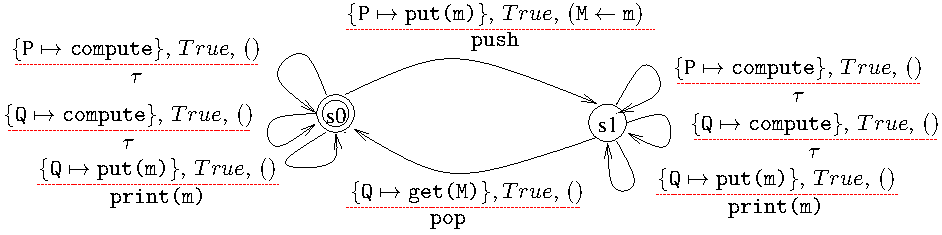
\includegraphics[width=.90\textwidth]{Figures/FIFOpen2.pdf}
   \caption{  The \texttt{simprod-cons} Open automaton: the system using one-place  buffer.  \label{Fig:SpecOA}}
\end{figure}
We can easily check that this automaton simulates the one of Fig.~\ref{Fig:RefineOA}.
Indeed, one can see that  $R=\{(r_0,s_0) \mapsto \texttt{l}=\texttt{f}, (r_0,s_1) \mapsto \texttt{f}=\texttt{l}+1\% \texttt{N} \}$ is  a candidate simulation 
relation. It follows that  \texttt{prod-cons} $\leq$ \texttt{simprod-cons}. \qed
\end{example}


%The refinement relation  also specifies that the refined process must follow the behaviour of the specification, not only at every compatible state but also along any scenario of the specification.


The refinement relation defined above is insufficient in the setting of composition which is the main advantage of the OA-based approach. Indeed, it should be possible to refine an automaton by filling its hole, providing a concrete view of a part of the application that was not specified originally. 
More generally, it should be possible to relate automata that do not have the same holes because composition is a crucial part of system specification.
%Thus, we believe composition should also be a form of refinement and call this feature \emph{refinement through composition}.
However, filling holes can result in a system with more or less holes than the original system because the plugged subsystem can contain itself many holes.
Next section  defines  a more powerful refinement relation able to reason on automata with different sets of holes.


%Technically,  it expresses how the concepts from the abstract and the refined systems are linked together.






\section{A Refinement Relation that Takes Holes into Account}\label{sec:holes}

This section  extends the preceding relation to automata where the set of holes is not the same. Indeed, when composing the set of  holes changes, and for example we want to state whether the automaton after composition is a refinement of the original automaton or not.

\subsection{Deadlock Reduction, Reachability, and Composition}

%A notion that is often used in the context of refinement is the notion of deadlock reduction. This property considers that two states related by a given relation and states that if one state can do a transition, then the other can do a transition too. This notion is not much interesting in the general case as there is a priori no relation between the two transitions. However, when the relation that relates states is a simulation, this will relate the possible transitions and the deadlock reduction will become a valuable property.
\begin{comment}

Next definition states that if $T_2$ is not in a deadlock position then $T_1$ can do a transition but not necessarily with the same input values. This is very weak but sufficient when composed with the def  of simulation.

\TODO{remove this def}
\begin{definition}[Deadlock reduction]\label{def:dpwd}\\
Let \(\OAg[1]\) and \(\OAg[2]\) be two OAs.
A relation on OA configurations \(R: S_1 \times S_2 \to \rformulas[V_1 \uplus V_2]\) is deadlock reducing if  it satisfies the following\footnote{Note that variables of $T_1$ are existentially quantified in the proposition.}:
\begin{multline*}
 \forall \mpar{s_1, s_2} \in S_1 \times S_2,\\ V_1 \uplus V_2 \uplus \biguplus_\subbox{t_2 \in \fOT{s_2}} \fvars{t_2} \vdash \left(R\mpar{s_1, s_2} \wedge \bigvee_\subbox{t_2 \in \fOT{s_2}} \fguard{t_2} \implies \bigvee_\subbox{t_1 \in \fOT{s_1}} \fguard{t_1} \right)
\end{multline*}
\end{definition}

Because of the symbolic nature of OAs and their structure, in this definition,  the fact that a guard is true is sufficient to reason on the possible paths. This slightly simplifies the definition and makes the characterisation of transition that can be triggered very symbolic. An equivalent but more classical definition of deadlock reduction could be expressed as well. It states that if there is a transition that can be triggered in the first automaton, then there is a transition from the related state in the second automaton that can be triggered. This second definition is more verbose, in particular because of the multiple quantifiers over transitions and automaton state. The alternative definition is equivalent to this one when reasoning on a refinement relation (but not in general).
\end{comment}

Unfortunately, the deadlock reduction property in the definition of refinement is not compositional: the composition operator can itself introduce a deadlock. In other words, when filling the hole of two related automata with a third one, even if there is a deadlock reduction between the two original automata, there might not be a deadlock reduction in the composed ones. The same problem may arise when two related automata are composed in the same hole of a third one. 

This creates a conflict between deadlock reduction and the properties involving composition. 
%One possible solution to avoid this conflict is to only consider a composition that do not introduce deadlocks, we  define such a composition below.
%But before defining non-blocking composition, we first introduce a notion of state reachability for open automata. 
%\begin{definition}[Reachability] \label{Def:Reach}
%For any open automata \(A = \OAg\), a reachability predicate \(\reach{A}: S \to \rformulas[V]\) is any predicate on states that is valid on initial state, and preserved across transitions:
%\[\sigma_0 \vdash \reach{A}\mpar{s_0}\quad\land\quad\forall t = \OTg \in T, \fvars{t} \vdash \left(\reach{A}\mpar{s} \wedge g \implies \reach{A}\mpar{s'}\psubst{\psi}\right)\]
%\end{definition}
%Reachability takes into account all paths, and can over-approximate the reachable configurations. 
%From an automation point of view, finding the most precise reachability predicate for a given automata is not decidable because of the symbolic nature of open automata, but only an over-approximation is necessary. An automatic tool would only need to find an over approximation of reachability to reason on composition that is compatible with deadlock reduction. 
We call \emph{non-blocking composition} a composition that can  safely be used to compose OA that are involved in a deadlock reducing relation.

%\begin{definition}[Non-blocking composition] \label{Def:Non-block}
%Let \(A_i = \OAg[i]\) with \( 0 \leq i \leq n\) be a family of open automata.
%Let \(A = A_0\mdbrk{j_i \mapsto A_i \middle| 1 \leq i \leq n}\) and $A= \OAg$.
%
%The composition \(A_0\mdbrk{j_i \mapsto A_i \middle| 1 \leq i \leq n}\) is non-blocking if   \(A \) has a reachability predicate such that, for each reachable configuration, if there is a possible transition in \(A_0\) then there is a possible transition in \(A\):
%\begin{multline*}
% \forall s = \mpar{s_0, s_1,..,s_n} \in S, V \uplus \biguplus_\subbox{t_0 \in \fOT{s_0}} \fvars{t_0} \vdash \\ \left(\reach{A}\mpar{s} \wedge \bigvee_\subbox{t_0 \in \fOT{s_0}} \fguard{t_0} \implies \bigvee_\subbox{t \in \fOT{s}} \fguard{t} \right)
%\end{multline*}
%\end{definition}
\begin{definition}[Non-blocking composition] \label{Def:Non-block}
Let \(A_1 \defobject \OAg[1]\) and \( A_2 \defobject \OAg[2]\) be two OA.
Let $A= \OAg$ be the OA resulting from the composition \(A = A_1\subst{A_2}{k}\). 
The composition \(A_1\subst{A_2}{k}\) is non-blocking if   \(A \) has a reachability predicate such that, for each reachable configuration, if there is a possible transition in \(A_1\) then there is a possible transition in \(A\):
\begin{multline*}
 \forall s = \mpar{s_1, s_2} \in S, V \uplus \biguplus_\subbox{t \in \fOT{s_1}} \fvars{t} \vdash  \left(\reach{A}\mpar{s} \wedge \bigvee_\subbox{t \in \fOT{s_1}} \fguard{t} \implies \bigvee_\subbox{t \in \fOT{s}} \fguard{t} \right)
\end{multline*}
\end{definition}
Like in the definition of refinement (Definition~\ref{def:HoleEqualSim}) we use guards to ensure that the transition can occur. 
In general, one would not want to only consider non-blocking composition as it may reveal a bit restrictive, but it is the best necessary condition that can be identified for compositionality of refinement. It will be used to prove composition theorems in  Section~\ref{sec:prop}. 
Proving refinement relation in absence of non-blocking composition may also checked specifically for the composed automaton under study.
%It is not sufficient to ensure the existence of equivalent transitions in general, but it will be sufficient in the context of refinement.



\subsection{Automaton refinement}

One major challenge in the extension of refinement to different sets of holes is to maintain a form of transitivity while being able to take into account the actions of some of the holes. A naive definition of refinement would ensure that only the holes that are identical in the two OA are taken into account in the simulation. Unfortunately considering all the common holes does not ensure transitivity of the simulation for the following reason. If $A_1$ simulates $A_2$ and $A_2$ simulates $A_3$, and one hole $j$ appears in $A_3$ and in $A_1$ but not in $A_2$ then we have no guarantee on the way $A_1$ and $A_3$ take the actions of this his hole into account, thus  a refinement between and $A_1$ and $A_3$ would require conditions involving actions of the hole $j$ which cannot be ensured. The way we solve this issue is to remember in the simulation relation which holes have been compared. This makes the relation parameterized by a subset of the set of holes that belong to the two automata that we want to take into account.
This way, in the example above, we would have no guarantee on actions the hole $j$ by transitivity but can state a refinement relation with guarantees on the actions of the other holes.

In the following definition we add a parameter $H$ which is the set of holes tracked by the refinement relation and adapt the definition by ignoring actions of the holes that are not in $H$.
\begin{definition}[Hole-tracking simulation]\label{Def:OA-Refinement}
For two OA\\ \(A_1 \defobject \OA{S_1}{s_{01}}{J_1}{V_1}{\sigma_{01}}{T_1}\) and \(A_2 \defobject \OA{S_2}{s_{02}}{J_2}{V_2}{\sigma_{02}}{T_2}\), \(A_1\) is a refinement of \(A_2\) tracking holes \(H\), noted \(\wrel{A_1}{A_2}{H}\), with \(H \subseteq J_1 \cap J_2\), if there is a relation on configurations $R: \mpar{S_1 \times S_2} \to \rformulas[V_1 \uplus V_2]$ such that:
\item[(1)] \(\sigma_{01} \uplus \sigma_{02} \vdash R\mpar{s_{01}, s_{02}}\)
\item[(2)] \(\forall \mpar{s_1, s_2} \in S_1 \times S_2,\)
\begin{multline*}
	\everymath{\displaystyle}\begin{array}{l}
		\bigsymb{\forall} \OTx{1}{}{1}{1} \in \fOT{s_1}, \bigsymb{\exists} \mpar{\OTx{2}{x}{2x}{2x} \in \fOT{s_2}}^{x \in X}, \\[12pt]
		\quad \mpar{\forall x \in X, J'_{2x} \cap H = J'_1 \cap H} \nwedge\\[1pt]
		 V_1 \uplus V_2 \uplus \fvars{t_1} \vdash\\\hspace{5em} \mpar{R\mpar{s_1, s_2} \wedge g_1 \implies \operatorname*{\bigsymb{\bigvee}}_{x \in X} \mpar{\begin{array}{l}
			\alpha_1 = \alpha_{2x} \wedge \bigwedge_\subbox{j \in J'_{2x} \cap H} \beta_{1j} = \beta_{2xj}   \nwedge\\
			 g_{2x} \wedge R\mpar{s'_1, s'_{2x}}\psubst{\psi_1 \uplus \psi_{2x}}
		\end{array}}} 
	\end{array} 
\end{multline*}
\item[(3)] Deadlock reduction:
\[
\forall \mpar{s_1, s_2} \in S_1 \times S_2, V_1 \uplus V_2  \vdash R\mpar{s_1, s_2} \implies( \bigvee_\subbox{t_1 \in \fOT{s_1}} \fguard{t_1} ) \lor¢ \lnot( \bigvee_\subbox{t_2 \in \fOT{s_2}} \fguard{t_2}  )
\]
\end{definition}
Note that every action of the holes outside \(H\) is unconstrained according to the refinement relation.

%\begin{example} It is easy to see the  open automaton of Fig.~\ref{Fig:RefineOA} is a refinement the open automaton of Fig.~\ref{Fig:SpecOA} according to this definition.
%\end{example}

\begin{property}[Relating simulations]\label{lem-sim-sim}
Hole-equal simulation is a particular case of hole-tracking refinement when  $J_1=J_2=H$.
\end{property}
\begin{example} Consider the automata of examples \ref{Example:fifo-system} and \ref{example:fifo-system-one}. As we saw above, \texttt{prod-cons} $\leq$ \texttt{simprod-cons}, therefore \texttt{prod-cons} $\leq_{\{\texttt{P,Q}\}}$ \texttt{simprod-cons}.
\end{example}
\TODO{potential ex 4: check if the example with a hole filled is a simulation of the example with holes? at least state \texttt{prod-cons} $\leq_{\{\texttt{P,Q}\}}$ \texttt{simprod-cons}}



%
%\TODO{
%A string $t \in \mathcal{A}^*$ is a trace of an automaton if there is some state $s$ such that $s_0 \xrightarrowdbl{t}  s$. We denote the set of traces of an automaton $A$ by $\mathcal{T}_A$. \\
%Notion of Extension refinement. May be we need to introduce the notion of  refusal of
%a trace $t \in \mathcal{T}_A$ is a set of actions such that all actions in the set can be refused after the automaton $A$
%has executed the trace $t$. \[X \in \bot_{A}(t) \Leftrightarrow \{\exists s. s_0  \xrightarrowdbl{t} s \wedge \forall a \in X. s \not{\xrightarrow{a}}    \}\] and replace deadlock reducing, under (3) by
%\[\forall t \in \mathcal{T}_{A_1} \cap  \mathcal{T}_{A_2},\, \bot_{A_2}(t) \subseteq  \bot_{A_1}(t)  \] } 
%
%\TODO{thm: backward compatibility + simulation is equivalent to extension refinement in case there is no hole and no guard, i.e. in case the definitions of automata coincide}

\begin{property}[Tracked holes] By construction, if an automaton is the refinement of another one, it is also a refinement by tracking less holes.
\[\wrel{A_1}{A_2}{H} \land H'\subseteq H \implies \wrel{A_1}{A_2}{H'}\]
\end{property}

Now that we have a refinement relation that takes both variable parameters and process parameters into account, we would like to ensure that it has  properties one would expect for a refinement relation.

\section{Properties of our Refinement Relations}\label{sec:prop}

We now  state the properties of our refinement relations, proofs of the properties can be found in the appendices. We express these properties in terms of hole-tracking simulation because, thanks to Property~\ref{lem-sim-sim}   all the properties  of hole-tracking simulation are also valid  for hole-equal simulation
The first crucial property of  refinement  is that it is  a  preorder on the set of OA. This property enables stepwise refinement.


\begin{theorem}[Simulation is a preorder]
Hole-tracking simulation
   is reflexive  and  transitive:  it  is  a  preorder on the set of OA.
\end{theorem}

\begin{proofsketch}
% TODO: I don't understand this definition, why v = v on vars(s1), what about s2
% ANS: was copy paste from the report, polished now
The relation  \(\wrel{}{}{H}\) is reflexive,  \(\wrel{A}{A}{H}\). This is shown  by considering the relation $R$ such that $R\mpar{s_1, s_2} \triangleq s_1=s_2\land \displaystyle\bigwedge_\subbox{v \in vars(s_1)} {v=v}$   we can prove the conditions for Definition~\ref{Def:OA-Refinement}.
%
%\begin{theorem}[Transitivity]
%If $\wrel{A_1}{A_2}{H}$ and $\wrel{A_2}{A_3}{H'}$, then $\wrel{A_1}{A_3}{H\cap H'}$.
%\end{theorem}
Appendix~\ref{sec:proof-transitivity} presents the proof of transitivity. It is done classically by identifying the relation between $A_1$ and $A_3$ that is a refinement. What is less classical is the definition of this relation because it is a boolean formula. For each couple of states  $s_1$ and $s_3$ of $A_1$ and $A_3$ we build a  formula that defines the refinement relation. To do this, we take the disjunction of formulas relating $s_1$ and $s_3$, and passing by all states $s_2$ of $A_2$. More precisely, we define a relation of the following form:
  \[R_{13}(s_1,s_3)=\bigvee_{s_2\in S_2}\mpar{R_{12}(s_1,s_2) \land R_{23}(s_2,s_3) } \]
We then prove that this relation  is a refinement, according to Definition~\ref{Def:OA-Refinement}.

\end{proofsketch}

The next  theorem states that if two automata are in refinement relation and the same automaton is placed in the same hole of the two automata, then the refinement is preserved. This is the first step toward proving that
 refinement is compositional in the sense that it is sufficient to prove refinement for the composed automata separately to obtain a refinement relation.
The second part,  proving that placing in the same context two OA in refinement, we obtain two OA in refinement is left for future works.
%
%
%The composition of $A_1$ and $A_3$ is a refinement of the composition of $A_2$ and $A_3$ provided $A_1$ is a refinement of $A_2$ and the hole in which we are composing inside $A_1$ and $A_2$ is tracked by the refinement relation.



\begin{theorem}[Context refinement]\label{thm:ContextRefinement}
Let $A_1$, $A_2$ and $A_3$ be three OA with $\wrel{A_1}{A_2}{H}$. 
Let $J_3$ be the set of holes of $A_3$ and suppose that $k \in H$.
Suppose additionally that  \(A_1\subst{A_3}{k}\) is non-blocking.
We have: \[\wrel{A_1\subst{A_3}{k}}{A_2\subst{A_3}{k}}{J_3 \uplus H \setminus \mbrc{k}}\]
\end{theorem}



%
%
%
%
%\begin{theorem}[Congruence]\label{thm:Congruence}
%Let $A_1$, $A_2$ and $A_3$ be three open automata with $\wrel{A_2}{A_3}{H}$. 
%%Suppose that \(k \in H\) and that \(A_1\subst{A_2}{k}\) is non-blocking.
%We have: \[\wrel{A_1\subst{A_2}{k}}{A_1\subst{A_3}{k}}{J_1 \uplus H \setminus \mbrc{k}}\]
%\end{theorem}

%\TODO{i did not put the global composition theorem, de we state it?}


\begin{proofsketch}
The proof relies on a simulation relation that we consider is the one that makes $A_1$ and $A_2$ similar, complemented with identity of configurations for $A_3$.
Then, by construction, all transitions of the composed automaton $A_1\subst{A_3}{k}$ are specified by open transitions of $A_1$. For the transitions that do not involve hole $k$, the transition of $A_1\subst{A_3}{k}$ is the same and simulation between $A_1$ and $A_2$ allows us to conclude directly. If the hole $k$ is involved the considered relation  implies that valuations in $A_3$ are equal (i.e., the value for each variable are the same in both valuations), after a transition we should obtain ``equal'' valuations because post-conditions are deterministic.
\end{proofsketch}

\begin{example}  Consider again the \texttt{prod-cons} and \texttt{simprod-cons}  automata given in the examples above.  Since  \texttt{prod-cons} $\leq_{\{\texttt{P,Q}\}}$ \texttt{simprod-cons},  then according to Theorem \ref{thm:ContextRefinement}, 
\texttt{prod-cons[producer/P]} $\leq_{\{\texttt{Q}\}}$  \texttt{simprod-cons[producer/P]}. 
The automaton of \texttt{prod-cons[producer/P]} is shown in Fig.~\ref{Fig:ComposeOA}.
The automaton resulting  from the composition of  \texttt{Simprod} and \texttt{producer} is bigger and not shown here. \qed
\end{example}


\begin{theorem}[Congruence]\label{thm:CongurenceRefinement}
Let $A_1$, $A_2$ and $A_3$ be three OA with $\wrel{A_2}{A_3}{H}$. 
  Let $J_1$ be the set of holes of $A_1$ and suppose that \(k \in J_1\). Suppose additionally that the composition $A_1\subst{A_2}{k}$ is non-blocking.
We have: \[\wrel{A_1\subst{A_2}{k}}{A_1\subst{A_3}{k}}{J_1 \uplus H \setminus \mbrc{k}}\]
\end{theorem}

Consequently, as the simulation is transitive \TODO{TODO Thm 4}
We can state the following theorem: 
\begin{theorem}[Composability]\label{thm:Composability}
Let $A_1$, $A_2$, $A_3$ and $A_4$ be four OA with $\wrel{A_1}{A_2}{H}$ and $\wrel{A_3}{A_4}{H'}$.  Suppose that \(k \in H\). We have: \[\wrel{A_1\subst{A_3}{k}}{A_2\subst{A_4}{k}}{ H \uplus H'\setminus \mbrc{k}}\]
\end{theorem}

\begin{example}
As an example of the use of this theorem, if we design a refined version of the producer process of Example~\ref{Example:prodandcons} called $\texttt{Refproducer}$. According to  Theorem \ref{thm:Composability}, we have 
\texttt{prod-cons[producer/P]} $\leq_{\{\texttt{Q}\}}$  \texttt{simprod-cons[$\texttt{Refproducer}$/P]}. 
%as well as \texttt{prod-cons[P/producer]} $\leq_{\{\texttt{Q}\}}$  \texttt{Simprod-cons[P/$\texttt{producer}^{\flat}$]}.
\end{example}


%\begin{figure}[h]
% \centering
%   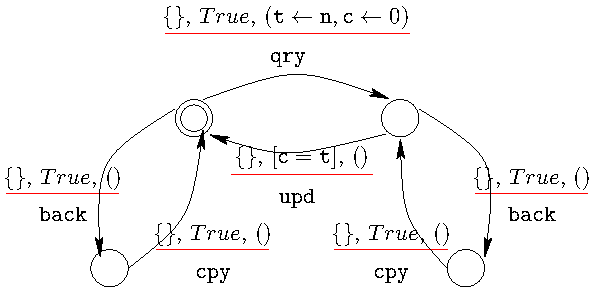
\includegraphics[width=.6\textwidth]{Figures/composeRefined.pdf}
%   \caption{Open automata resulting from the composition of the  refined  \texttt{database} and the \texttt{counter} \label{Fig:ComposeRefine}}
%\end{figure}



% TODO: why is there several ovoid stacked only on one side?
%\begin{center}
%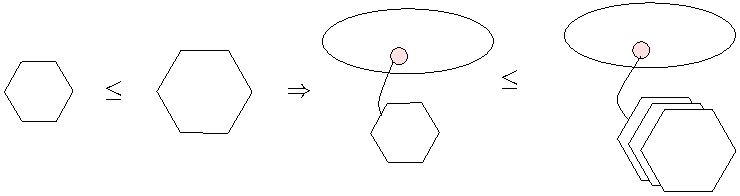
\includegraphics[scale=0.7]{Figures/Theorem1}
%\end{center}

%% TODO: non-blocking is not defines afaik
%% ANS: remove this from the submission because proof unfinished
%Open automata composition is a refinement where
%the tracked holes are the holes of the base automaton minus the composed hole.
%\begin{theorem}[Composition is a refinement]\label{thm:Composition}
%Let $A_1$ and  $A_2$  be three two automata with $J_1$ the set of holes of $A_1$.
%Suppose that \(k \in J_1\) and that \(A_1\subst{A_2}{k}\) is non-blocking. We have:
%\[ \wrel{A_1\subst{A_2}{k}}{A_1}{J_1\setminus \{k\}}\]
%\end{theorem}


%TODO: FOCUS on the two following items (look at quentin's article):
%
%
%- what is the property wrt deadlocks?
%
%
%- relation with fh bisimulation

Note that the substitution operation can be extended to a multiple substitution that fills several holes at the same time, and the theorems can be adapted accordingly.

%\TODO{parler de generalisation a la composition a n automates}

\section{Related Work}
\label{sec:sota}



There are some works that have focused on  the refinement of open systems. Defining refinement of open systems as trace inclusion  is  addressed  as a notion of subtyping in type theory 
\cite{GayH:2005,BravettiZ:2021}. This kind of refinement is  based  on interface-oriented approach, it allows the expression of more internal choices and less external choices. The refinement of open systems is also defined in terms of  alternating simulation \cite{Alur:1998,deAlfaro:2021}, which deals with game-based models.
Alternating simulation that is originating from the game theory \cite{deAlfaro:2003} allows  the study of relation between individual components by viewing them as alternating transition systems. In particular,  a refinement of game-based automata expresses that the refined component can offer more services (input actions) and fewer service demands (output actions). However, the composition of such automata may
lead to illegal states, where one automaton issues an output that is not acceptable as input in the other one. The theory of alternating simulation provides an optimistic approach to compute compatibility between automata based on the fact that each automaton expects the other to provide  legal inputs, i.e, two components can be composed if there is an environment where they can work together. As we shall see in this paper, 
our approach to design refinement  has some commonalities with that of the above mentioned \cite{deAlfaro:2021}: both are process-oriented approach even if they are not based on the same notion of simulation and they are based on optimistic approach to composition. 
For the composability, we use the notion of comparability of holes (similar to the notion of compatibility), which is explicitly encompassed in the definition of composition.

 



Previous works on OA focused on equivalence relations compatible with composition.
In  \cite{10.1145/3372884.3373161}, a computable bisimulation is introduced, while in \cite{fhbisim} is introduced a weak version of the bisimulation on OA. 
In this paper we tackle the refinement relation in the form of simulation, as is the case for the corresponding relations on labelled transition systems \cite{10.1007/3-540-46428-X_19}. But unlike the standard simulation we deal with symbolic and open models. In \cite{Zhang2014}, the authors exploit transition systems to reason about the systems  that are partially specified by using variables, making  the state space potentially infinite.

The simulation  ensures the preservation of   
safety properties as deadlock-freeness  and, more generally, 
all linear temporal logic properties.  Our focus is about the properties of simulation, in particular closure properties such as preservation under composition. Some works   have addressed the problem of non-introduction of blocking by composition. For example, in \cite{DIHEGO2020110598} it is presented a refinement relation on process algebra based on failure semantics that is basically different from the (bi)simulation \cite{10.5555/640428.640430}.   
  
 





\section{Conclusion}\label{sec:ccl}
In this article we investigated the notion of refinement for a symbolic and open model: open automata. 
OA are convenient to model parallel systems that are parameterised both by the use of variables and by the possibility to compose automata.
The refinement relation first relies on a simulation relation between the specification and its refinement, but it also specifies that the refined process must follow the behaviour of the specification, not only at every compatible state but also along any trace.
We finally showed that refinement is a preorder that is preserved when filling a hole.

In the future we will focus on the other composition property that considers the preservation of refinement when automata are placed in the same context, namely filling the hole of the same automaton by an automaton and its refinement. This property should require some restriction on the composed processes.
 Finally, we will investigate under which condition, the composition operation produces a refinement in the sense that filling a hole produces a refined process.




 \bibliographystyle{splncs04}
 \bibliography{biblio}

\newpage

\appendix


\section{Proof of Transitivity for Refinement}\label{sec:proof-transitivity}
\begin{quote}
If $\wrel{A_1}{A_2}{H}$ and $\wrel{A_2}{A_3}{H'}$, then $\wrel{A_1}{A_3}{H\cap H'}$.
\end{quote}

\proof 
If $\wrel{A_1}{A_2}{H}$ then there is $R_{12}$ a relation between states
of $A_1$ and of $A_2$;  If $\wrel{A_2}{A_3}{H'}$ then there is $R_{23}$ a relation between states of $A_2$ and of $A_3$. We build a relation between
 states of $A_1$ and of $A_3$ as follows:  for each pair of states $s_1$, $s_3$, for each state $s_2$ such that $R_{12}$ relates $s_1$ and $s_2$, and $R_{23}$ relates $s_2$ and $s_3$.
Let $R_{13}$ be the relation:\\
  \[R_{13}(s_1,s_3)=\bigvee_{s_2\in S_2}\mpar{R_{12}(s_1,s_2) \land R_{23}(s_2,s_3) } \]

We will show that $\wrel{A_1}{A_3}{H\cap H'}$ by exhibiting  $R_{13}$ as a hole-tracking simulation of $A_1$ by  $A_3$.

We have to prove that the relation $R_{13}$ satisfies the three conditions of the definition of a refinement of OA.
\begin{enumerate}
\item Firstly, we have to $R_{13}$ satisfies initial configurations:
\[\sigma_{01} \uplus \sigma_{03} \vdash R_{13} \mpar{s_{01}, s_{03}}\]
By knowing that substitutions only have an effect on the variables of the OA they belong to, they also produce terms containing only variables of the OA they belong to. We have:
\begin{align*}
\mpar{\sigma_{01} \uplus \sigma_{02} \vdash R_{12}\mpar{s_{01}, s_{02}}} \wedge \mpar
{\sigma_{02} \uplus \sigma_{03} \vdash R_{23}\mpar{s_{02}, s_{03}}}&\implies\\
R_{12}\mpar{s_{01},s_{02}}\psubst{\sigma_{01} \uplus \sigma_{02}} \wedge R_{23}\mpar{s_{02}, s_{03}}\psubst{\sigma_{02} \uplus \sigma_{03}}&\implies\\
R_{12}\mpar{s_{01},s_{02}}\psubst{\sigma_{01} \uplus \sigma_{02} \uplus \sigma_{03}} \wedge R_{23}\mpar{s_{02}, s_{03}}\psubst{\sigma_{01} \uplus \sigma_{02} \uplus \sigma_{03}}&\implies\\ 
\underbrace{R_{12}\mpar{s_{01},s_{02}}\wedge R_{23}\mpar{s_{02}, s_{03}}}_{\implies R_{13} \mpar{s_{01}, s_{03}}}\psubst{\sigma_{01} \uplus \sigma_{02} \uplus \sigma_{03}} %&\implies\\
 \end{align*}
Since $\sigma_{02}$ has no effect on variables of $s_{01}$ and $s_{03}$ thus we get the expected result.

\item \TODO{Ref to JLAMP 2023?}

\item Lastly, we have to prove the satisfaction of the deadlock reduction condition. 
 To build $R_{13}$ we need to rely on the disjunction of all possible paths to relate $s_1$ and $s_3$, which leads to \[{\displaystyle R_{13}(s_1,s_3)=\bigvee_{{p\in P}}\mpar{R_{12}\mpar{s_1,s_{2p}} \wedge R_{23}\mpar{s_{2p},s_3}}}\]

Consider any $\mpar{s_{1}, s_{3}} \in R_{13}$  there is a set of states $(s_{2p})^{p\in P}$ of $A_2$ relating  $s_{1}$ and $s_{3}$.


First, according to the relation between $A_1$ and $A_2$ OA,  for all $\mpar{s_1, s_{2p}} \in S_1\times S_2$  we have:
\begin{multline*}
%\forall \mpar{s_1, s_{2p}} \in S_1 \times S_2, 
V_1 \uplus V_2  \vdash R_{12}\mpar{s_1, s_{2p}} \implies \bigvee_\subbox{t_1 \in \fOT{s_1}} \fguard{t_1}  \lor¢ \lnot( \bigvee_\subbox{t_{2p} \in \fOT{s_{2p}}} \fguard{t_{2p}}  )
\end{multline*}
Second, according to the relation between $A_2$ and $A_3$ OA, for all $\mpar{s_{2p},s_3} \in S_2\times S_3$  we have:
\begin{multline*}
 V_2 \uplus V_3  \vdash R_{23}\mpar{s_{2p},s_3} \implies  \bigvee_\subbox{t_1 \in \fOT{s_{2p}}} \fguard{t_{2p}}  \lor¢ \lnot( \bigvee_\subbox{t_3 \in \fOT{s_3}} \fguard{t_3} )
\end{multline*}
With the conjunction of both, we get:

\begin{multline*}
 V_1 \uplus V_2 \uplus V_3  \vdash  R_{12}\mpar{s_1, s_{2p}} \wedge R_{23}\mpar{s_{2p},s_3} \implies   \bigvee_\subbox{t_1 \in \fOT{s_1}} \fguard{t_1} 
 \lor¢ \lnot( \bigvee_\subbox{t_3 \in \fOT{s_3}} \fguard{t_3} )
\end{multline*}


This is valid for all $s_{2p} \in (s_{2p})^{p\in P}$, then we have:
\begin{multline*}
 V_1 \uplus V_2 \uplus V_3  \vdash \underbrace{\bigvee_{{p\in P}}\mpar{R_{12}\mpar{s_1, s_{2p}} \wedge R_{23}\mpar{s_{2p},s_3}}}_{R_{13}(s_1,s_3)} \implies  ( \bigvee_\subbox{t_1 \in \fOT{s_1}} \fguard{t_1} )
 \lor¢ \lnot( \bigvee_\subbox{t_3 \in \fOT{s_3}} \fguard{t_3} )
\end{multline*}
By removing the $A_2$ variables that have not effect on $A_2$ et $A_3$,
we get the desired result:
\begin{multline*}
 V_1 \uplus  V_3  \vdash R_{13}(s_1,s_3) \implies  ( \bigvee_\subbox{t_1 \in \fOT{s_1}} \fguard{t_1} )
 \lor¢ \lnot( \bigvee_\subbox{t_3 \in \fOT{s_3}} \fguard{t_3} )
\end{multline*}
\qed
\end{enumerate}
\section{Proof of Context Refinement (Theorem~\ref{thm:ContextRefinement})}



\begin{quote}
Suppose that $\wrel{A_1}{A_2}{H}$, \(k \in H\) and that \(A_1\subst{A_3}{k}\) is non-blocking. We have: 
\[\wrel{A_1\subst{A_3}{k}}{A_2\subst{A_3}{k}}{J_3 \uplus H \setminus \mbrc{k}}\]
\end{quote}
\smallskip
Pictorially, the theorem states the following result:

\begin{center}
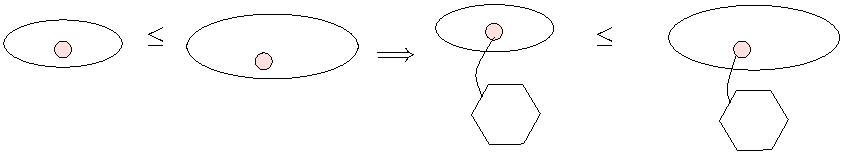
\includegraphics[scale=0.7]{Figures/Thm2intuition}
\end{center}

\proof
Let us denote by $A_{13}$ (resp. $A_{23}$) the OA resulting from $A_1\subst{A_3}{k}$ (resp. $A_2\subst{A_3}{k}$),  to prove the theorem it is sufficient to prove that there exists a relation between states of the two OA that satisfies the conditions of the Definition \ref{Def:OA-Refinement}. 

We denote $A_1=  \OA{S_1}{s_{01}}{J_1}{V_1}{\sigma_{01}}{T_1}$ and \(A_2 \defobject \OA{S_2}{s_{02}}{J_2}{V_2}{\sigma_{02}}{T_2}\) and $A_3 = \OA{S_3}{s_{03}}{J_3}{V_3}{\sigma_{03}}{T_3}$. The proof requires  to rename the variables of one instance of the two $A_3$ automata to avoid clashes in variable names (this is required by the definition of refinement). In practice we will use superscripts ${}^1$ and ${}^2$ to distinguish elements of the two instances of $A_3$.

Let $R$ be the refinement relation relating states of $A_1$ and $A_2$. 
Let us denote with $t^1$ and $t^2$  the elements of $A_1$ and $A_2$ respectively.
Consider any two states $s_{13} = \mpar{s_1,s^1_3}$ and $s_{23} = \mpar{s_2,s^2_3}$ ($s^1_3$ and $s^2_3$  are the same with renaming). We define a relation $R'$ relating states of $s_{13}$ and $s_{23}$ as follows:
\[ R' \mpar{s_{13}, s_{23}} = R\mpar{s_{1}, s_{2}} \land \reach{A_{13}}(s_{13})  %\wedge \reach{A_{13}}\mpar{s_{13}}
 \wedge \bigwedge_\subbox{v_3\in V_3}
 v^1_3=v^2_3\land s^1_3 = s^2_3\]

%\TODO{[Ludo] I believe reachability is not useful here -- to check}

We want to prove that $\mpar{R', H\uplus J_3 \setminus\{k\}}$ is a hole-tracking simulation of $A_{13}$ and $A_{23}$. In the following we denote $H'=H\cup J_3 \setminus\{k\}$.
\begin{enumerate}
\item First, we have to prove the relation for initial states:
\[\sigma_{013} \uplus \sigma_{023} \vdash R'\mpar{s_{013}, s_{023}}\]
with $\sigma_{013} = \sigma_{01} \uplus \sigma_{03}^1$, $\sigma_{023} = \sigma_{02} \uplus \sigma_{03}^2$, $s_{013}=(s_{01},s_{03}^1)$, and $s_{023}=(s_{02},s_{02}^2)$.\\
By using the fact that $R$ relates initial configurations of  $A_1$ and $A_2$, we have:
$\mpar{\sigma_{01} \uplus \sigma_{02} \vdash R\mpar{s_{01}, s_{02}}}$.  
%and based on the  fact that initial states are reachable $\sigma_{013} \vdash \reach{A_{13}}\mpar{s_{013}}$ we have 
%\[ \mpar{\sigma_{01} \uplus \sigma_{02} \vdash R\mpar{s_{01}, s_{02}}} \wedge 
%\mpar{\sigma_{013} \vdash \reach{A_{13}}\mpar{s_{013}}}\]

Considering that initial valuations $\sigma_{03}^1$ and $\sigma_{03}^2$ associate the same values to the ``same'' variables modulo renaming, so the following holds:\\ $\left(\,\,{\displaystyle \bigwedge_\subbox{v_3\in V_3} v^1_3=v^2_3\wedge s^1_3 = s^2_3}\right)\psubst{\sigma_{03}^1 \uplus \sigma_{03}^2 }$.

Additionally, because  the domains of the substitution function are disjoint, the substitution function has an effect only on the related elements,  we get:
\begin{align*}
& \mpar{\sigma_{01} \uplus \sigma_{02} \vdash R\mpar{s_{01}, s_{02}}} 
%\wedge \mpar{\sigma_{013} \vdash \reach{A_{13}}\mpar{s_{013}}}
\\
\implies & R\mpar{s_{01}, s_{02}}\psubst{ \sigma_{01} \uplus \sigma_{02}}  \land \mpar{\,\,\bigwedge_\subbox{v_3\in V_3} v^1_3=v^2_3\wedge s^1_3 = s^2_3}\psubst{\sigma_{03}^1 \uplus \sigma_{03}^2 }\\
\implies & \mpar{R\mpar{s_{01}, s_{02}} \wedge  \bigwedge_\subbox{v_3\in V_3}  v^1_3=v^2_3\wedge s^1_3 = s^2_3} \psubst{ \sigma_{01} \uplus \sigma_{02} \uplus \sigma^1_{03}\uplus \sigma^2_{03}\uplus \sigma_{013} }\\
\implies & \sigma_{013} \uplus \sigma_{023} \vdash R'\mpar{s_{013}, s_{023}}
\end{align*}
The last step comes from the additional fact that  $\reach{A_{13}}(s_{013})$.

\item Second, we need to prove for any open transition $t_{13}$ in $T_{13}$ originating from $s_{13}$:
\begin{align*}
		&  \OTx{13}{}{13}{13} \in \fOT{s_{13}}
\end{align*}		
there exists an indexed family $t_{23x}$ of OTs originating from $s_{23}$ that simulate it: 
\begin{align*}
		&  \mpar{\OTx{23}{x}{23x}{23x} \in \fOT{s_{23}}}^{x \in X}
\end{align*}	
\begin{align*}		
		& \text{such that } \mpar{\forall x \in X, J'_{23x} \cap H' = J'_{13} \cap H'} \text{ and }\\
		&  V_{13} \uplus V_{23} \uplus \fvars{t_{13}} \vdash\\
		& R'\mpar{s_{13}, s_{23}} \wedge g_{13} \implies \operatorname*{\bigsymb{\bigvee}}_{x \in X} \mpar{\everymath{\displaystyle}\begin{array}{l}
			\alpha_{13} = \alpha_{23x} \wedge \bigwedge_\subbox{j \in J'_{23x} \cap H'} \beta_{13j} = \beta_{23xj} \wedge\\[12pt]
			 g_{23x} \wedge R'\mpar{s'_{13}, s'_{23x}}\psubst{\psi_{13} \uplus \psi_{23x}}
		\end{array}} 
	\end{align*}


Recall that by definition of composition and OA refinement we have: 
\begin{align*}
&V_{13}= V_1\uplus V^1_3 \text{ and }
V_{23}= V_2\uplus V^2_3\\
& H' \subseteq J_3\uplus \mpar{J_1 \cap J_2} \setminus \{k\} = \mpar{J_3\uplus J_1 \setminus \{k\} } \cap \mpar{J_3\uplus J_2 \setminus \{k\}} \\
\end{align*}
First of all, we have by hypothesis $\wrel{A_1}{A_2}{H}$, then for any open transition $t_1$ in $T_1$  originating from $s_1$:
\begin{align*}
\OTx{1}{}{1}{1} \in \fOT{s_1}
\end{align*}
there exists an indexed family of OTs originating from $s_{2}$: 
\begin{align*}
\mpar{\OTx{2}{x}{2x}{2x} \in \fOT{s_{2}}}^{x \in X} 
\end{align*}
such that $\forall x \in X, J'_{2x} \cap H = J'_1 \cap H$ and
\begin{multline*}
%\everymath{\displaystyle}
V_1 \uplus V_2 \uplus \fvars{t_1} \vdash\\ \mpar{R\mpar{s_1, s_{2}} \wedge g_1 \implies \operatorname*{\bigsymb{\bigvee}}_{x \in X} \mpar{\everymath{\displaystyle}
\begin{array}{l}
			\alpha_1 = \alpha_{2x} \wedge \bigwedge_\subbox{j \in J'_{2x} \cap H} \beta_{1j} = \beta_{2xj} \nwedge\\
			 g_{2x} \wedge R\mpar{s'_1, s'_{2x}}\psubst{\psi_1 \uplus \psi_{2x}}
		\end{array}}}  \qquad \quad (*)
\end{multline*}	
\smallskip

Consider any transition $t_{13}$ in $A_{13}$.  Based on  the definition of composition $t_{13}$ can be obtained from two different cases, we will consider the two cases separately. 


\paragraph{First case: Both automata perform a transition.}
The transition $t_{13}$ is obtained by the composition of  transitions $t_1=\OTx{1}{}{1}{1}\in \fOT{s_1}$ and  \[t_3^1=
\OT{ s^1_3}{{s^1_3}'}{\alpha_3^1}{   {(\beta^1_{3j})^{j \in J^{1 \prime}_3} }}{ g^1_3 }{ \psi^1_3}\in \fOT{s^1_3} \qquad \text{ when } k \in J'_{1} 
\] The result is:
\[
t_{13} = \OT{\mpar{s_1, s^1_3}}{\mpar{s'_1, {s^1_3}'}}{\alpha_1}{\beta_{1j}^{j \in J'_1 \setminus \{k\}} \uplus  {(\beta^1_{3j})^{j \in J^{1 \prime}_3} }}{g_1 \wedge g^1_3 \wedge \alpha^1_3 = \beta_{1k}}{\psi_1 \uplus \psi^1_3} \qquad \text{ where } k \in J'_{1} 
\]
We then obtain a family of OTs by the simulation of $A_1$ by $A_2$ (as stated above).
By hypothesis we have $k \in H$, so in the case where $k \in J'_{1}$, we deduce that $k \in J'_{2x}$ we can  then build  a family of OTs $t_{23x}^{x\in X}$ with the same transitions of $A_3$ (up to renaming) as those used to build $t_{13}$.
\[
t_{23x} = \left(\OT{\mpar{s_2, s^2_3}}{\mpar{s'_{2x}, {s^2_3}'}}{\alpha_{2x}}{\beta_{2xj}^{j \in J'_{2x}  \setminus \{k\}} \uplus   {(\beta^2_{3j})^{j \in J^{2 \prime}_3} }}{g_{2x} \wedge g^2_3 \wedge \alpha^2_3 = \beta_{2xk}}{\psi_{2x} \uplus \psi^2_3}
\right)^{x\in X}\]
Recall that in this case  $k \in J'_{1}$, so $\forall x \in X$ we have
\begin{align*}
  J'_{23x} \cap H'  
&=((J'_{2x}  \setminus \mbrc{k})\uplus J^{2 \prime}_{3} ) \cap (H\uplus J_3 \setminus\{k\} )\\
&=((J'_{2x}\cap (H\uplus J_3))\uplus (J^{2 \prime}_{3}\cap (H\uplus J_3)))\setminus \mbrc{k}\\
&=((J'_{2x}\cap H)\uplus (J^{2 \prime}_{3}\cap  J_3))\setminus \mbrc{k}\text{ since } J_3\cap J'_{2x} = \emptyset \text{ and } H\cap J^{2 \prime}_{3} = \emptyset\\
& =((J'_{2x}\cap H)\uplus J^{2 \prime}_{3})\setminus \mbrc{k}\text{ since } J^{2 \prime}_{3}\subseteq J_3\\
& =((J'_1\cap H)\uplus J^{1 \prime}_{3})\setminus \mbrc{k}\quad \text{ since } J^{1 \prime}_{3}=J^{2 \prime}_{3} \text{ and } J'_1 \cap H = J'_{2x} \cap H\\
&= ((J'_1 \cap H) \uplus (J^{1 \prime}_{3} \cap J_3)) \setminus \mbrc{k}\text{ since } J^{1 \prime}_{3}\subseteq J_3\\ 
& = (J'_1\cap (J_3 \uplus H)) \uplus ((J^{1 \prime}_{3} \cap (J_3 \uplus H)) \setminus \mbrc{k} \text{ since } J_3\cap J'_{1} = \emptyset \text{ and } H\cap J^{1 \prime}_{3} = \emptyset\\
		& = \mpar{(J'_1  \uplus J^{1 \prime}_{3})\setminus \mbrc{k}} \cap \mpar{(J_{3} \uplus H) \setminus \mbrc{k}}\\
		& = J'_{13} \cap H'
\end{align*}	

In this case the composition gives: \[g_{13} \Leftrightarrow g_1 \wedge g^1_3 \wedge \alpha^1_3=\beta_{1k} \text{ and }
g_{23x}  \Leftrightarrow g_{2x} \wedge g^2_3 \wedge \alpha^2_3=\beta_{2xk}\]
As $k \in H$ we have   
$\beta_{1k} = \beta_{2xk}$ then we  deduce:
\[g^1_3 \wedge \alpha^1_3=\beta_{1k}  \Leftrightarrow g^2_3 \wedge \alpha^2_3= \beta_{2xk}\]
The proof of the rest  is based on the following facts: 
\begin{enumerate}
\item  By construction of  $t_{13}$ and $t_{23x}$ we have $\alpha_{13}=
\alpha_{1}$ and $\alpha_{23x}=\alpha_{2x}$. So we deduce: 
$\alpha_{1} = \alpha_{2x} \Rightarrow \alpha_{13} = \alpha_{23x}$.
\item By composition we have also: \\ $\beta_{13j}^{j\in J'_{13}}= \beta_{1j}^{j \in J'_{1}  \setminus \{k\}} \uplus   {(\beta^1_{3j})^{j \in J^{1 \prime}_3} }$
and $\beta_{23xj}^{j\in J'_{23}}= \beta_{2xj}^{j \in J'_{2x}  \setminus \{k\}} \uplus   {(\beta^2_{3j})^{j \in J^{2 \prime}_3} }$\\
Therefore, we have for all $j\in J'_{13}$ (recall that $J'_{13}=J'_{23}$):  \[\beta_{13j} = \beta_{23xj} \Rightarrow (j\in J'_1 \land \beta_{1j} = \beta_{2xj}) \vee (j\in J_3^{1\prime} \land \beta^1_{3j}= \beta^2_{3j})\]
\item 
Considering $\beta^1_{3j}$ and  $\beta^2_{3j}$  are the same (up to renaming)  we have: \\
${\displaystyle V^1_{3} \uplus V^2_{3} \uplus \fvars{t_{13}} \vdash \bigwedge_\subbox{v_3\in V_3}\!\! v^1_3=v^2_3\implies \bigwedge_\subbox{j \in J^{2 \prime}_3} \beta^1_{3j}= \beta^2_{3j}}$\\
Then we compose by  disjunction with the following hypothesis (part of formula $(*)$).\\ $V_{1} \uplus V_{2} \uplus \fvars{t_1}  \vdash {\displaystyle \bigwedge_\subbox{j \in J'_{2x} \cap H} \beta_{1j} = \beta_{2xj}}$ 
\begin{align*}
 V_{1} \uplus V_{2}  \uplus V^1_{3} \uplus V^2_{3} \uplus \fvars{t_{13}}\vdash &    \bigwedge_\subbox{v_3\in V_3}\!\! v^1_3=v^2_3 \implies {\displaystyle \bigwedge_\subbox{j \in J'_{2x} \cap H} \beta_{1j} = \beta_{2xj}} \vee {\displaystyle \bigwedge_\subbox{j \in J^{2 \prime}_3} \beta^1_{3j}= \beta^2_{3j}}\\
\Rightarrow  V_{13} \uplus V_{23}  \uplus \fvars{t_{13}}\vdash & \bigwedge_\subbox{v_3\in V_3}\!\! v^1_3=v^2_3\implies {\displaystyle \bigwedge_\subbox{j \in (J'_{2x}   \cap H)\uplus J^{2 \prime}_3 } \beta_{13j} = \beta_{23xj}} \\  
\Rightarrow  V_{13} \uplus V_{23}  \uplus \fvars{t_{13}}\vdash & \bigwedge_\subbox{v_3\in V_3}\!\! v^1_3=v^2_3\implies {\displaystyle \bigwedge_\subbox{j \in    ((J'_{2x}   \cap H)\uplus J^{2 \prime}_3)\setminus \{k\} } \beta_{13j} = \beta_{23xj}} \\
\Rightarrow    V_{13} \uplus V_{23}  \uplus \fvars{t_{13}}\vdash & \bigwedge_\subbox{v_3\in V_3}\!\! v^1_3=v^2_3\implies {\displaystyle \bigwedge_\subbox{j \in (J'_{23x}   \cap H') } \beta_{13j} = \beta_{23xj}}
\end{align*}
\end{enumerate}

We can extend the valuation context of the variables to cover the variables of the transitions $t_3$ and the variables in $V_3^1$ and $V_3^2$ in the formula $(*)$.  
By   using the statements resulting from the cases (a), (b) and (c), we get:
\begin{multline*}
V_{13} \uplus V_{23}  \uplus \fvars{t_{13}} \vdash\\
R\mpar{s_1, s_{2}} \wedge \mpar{g_1 \wedge g^1_3 \wedge \alpha^1_3=\beta_{1k}}\wedge \bigwedge_\subbox{v_3\in V_3}  v^1_3=v^2_3 %\wedge s^1_3=s^2_3
\implies  \hspace{12em}\\
\operatorname*{\bigsymb{\bigvee}}_{x \in X} \mpar{\everymath{\displaystyle}
\begin{array}{l}
			\alpha_{13} = \alpha_{23x} \wedge \bigwedge_\subbox{j \in (J'_{23x} \cap H')} \beta_{13j}\! =\! \beta_{23xj}\nwedge\\
			  g_{2x} \wedge R\mpar{s'_1, s'_{2x}}\psubst{\psi_1 \uplus \psi_{2x}}
		\end{array}}  \wedge g^2_3 \wedge \alpha^2_3=\beta_{2xk} 
%\wedge \bigwedge_\subbox{v_3\in V_3}  v^1_3=v^2_3\wedge s^1_3=s^2_3
\end{multline*}	
That can be re-written as follows:
\begin{multline*}
V_{13} \uplus V_{23} \uplus \fvars{t_{13}}  \vdash\\
R\mpar{s_1, s_{2}} \wedge g_{13}  \land \bigwedge_\subbox{v_3\in V_3} v^1_3=v^2_3
\implies  \operatorname*{\bigsymb{\bigvee}}_{x \in X} \mpar{\everymath{\displaystyle}
\begin{array}{l}
			\alpha_{13} = \alpha_{23x} \wedge \bigwedge_\subbox{j \in J'_{23x} \cap H'} \beta_{13j} = \beta_{23xj} \nwedge\\
			g_{23x} \wedge R\mpar{s'_1, s'_{2x}}\psubst{\psi_1 \uplus \psi_{2x}}
		\end{array}}   
\end{multline*}	

Moreover, we have  for any transition $t_3$ in $A_3$ relating $s_3$ and $s^{\prime}_3$ the following:
\begin{multline*}
V_{13} \uplus V_{23}  \uplus \fvars{t_{13}} \vdash\\
\bigwedge_\subbox{v_3\in V_3}\!\! v^1_3=v^2_3  \wedge s^1_3 = s^2_3 \implies \bigwedge_\subbox{v_3\in V_3}\!\! \psi_{13}(v^1_3)=\psi_{13}(v^2_3)  \wedge s^{1\prime}_3 = s^{2\prime}_3 
\end{multline*}

 Furthermore,  according to the Definition \ref{Def:Reach} (reachability applied to the composed automaton ${A_1\subst{A_3}{k}}$) we have, for all $t_{13} \in T_{13}$:
\[ \fvars{t_{13}} \vdash \left(\reach{A_{13}}\mpar{s_{13}} \wedge g_{13} \implies \reach{A_{13}}\mpar{s_{13}'}\psubst{\psi_{13}}\right) \]	
Thus, we get:
\begin{multline*}
V_{13} \uplus V_{23} \uplus \fvars{t_1}  \cap \fvars{t_{13}} \vdash\\
R\mpar{s_1, s_{2}} \wedge g_{13}  {\wedge \reach{A_{13}}\mpar{s_{13}}}
\wedge \bigwedge_\subbox{v_3\in V_3}  v^1_3=v^2_3\wedge s^1_3=s^2_3
\implies \hspace{5em} \\ \operatorname*{\bigsymb{\bigvee}}_{x \in X} \mpar{\everymath{\displaystyle}
\begin{array}{l}
			\alpha_{13} = \alpha_{23x} \wedge \bigwedge_\subbox{j \in J'_{23x} \cap H'} \beta_{13j} = \beta_{23xj} \nwedge 	g_{23x} \wedge R\mpar{s'_1, s'_{2x}}\psubst{\psi_1 \uplus \psi_{2x}}\\
		  \wedge {\reach{A_{13}}\mpar{s_{13}'}\psubst{\psi_{13}} 
\wedge} \bigwedge_\subbox{v_3\in V_3}  \psi_{13}(v^1_3)=\psi_{13}(v^2_3)\wedge s^{1\prime}_3=s^{2\prime}_3
		\end{array}}   
\end{multline*}
	
From the two previous formulas, we get:
\begin{multline*}
V_{13} \uplus V_{23} \uplus \fvars{t_{13}}  \vdash\\
R\mpar{s_1, s_{2}} \wedge g_{13} \land {\reach{A_{13}}\mpar{s_{13}} \land} \bigwedge_\subbox{v_3\in V_3} v^1_3=v^2_3 \wedge s^1_3 = s^2_3
\implies \hspace{7em} \\ \operatorname*{\bigsymb{\bigvee}}_{x \in X} \mpar{\everymath{\displaystyle}
\begin{array}{l}
			\alpha_{13} = \alpha_{23x} \wedge \bigwedge_\subbox{j \in J'_{23x} \cap H'} \beta_{13j} = \beta_{23xj} \nwedge g_{23x}\land  {\reach{A_{13}}\mpar{s_{13}'}\psubst{\psi_{13}}}		\nwedge\\
			  R\mpar{s'_1, s'_{2x}}\psubst{\psi_1 \uplus \psi_{2x}} \wedge
 \bigwedge_\subbox{v_3\in V_3}\!\! \psi_{13}(v^1_3)=\psi_{13}(v^2_3) \wedge s^{1\prime}_3 = s^{2\prime}_3
		\end{array}}   
\end{multline*}

Because of the independence of the substitution domains, we simplify and get the expected formula:
	\begin{multline*}
  V_{13} \uplus V_{23} \uplus \fvars{t_{13}} \vdash\\ R^{\prime}\mpar{s_{13}, s_{23}} \wedge g_{13} \implies \operatorname*{\bigsymb{\bigvee}}_{x \in X} \mpar{\everymath{\displaystyle}\begin{array}{l}
			\alpha_{13} = \alpha_{23x} \wedge \bigwedge_\subbox{j \in J'_{23x} \cap H'} \beta_{13j} = \beta_{23xj} \nwedge\\[12pt]
			 g_{23x} \wedge R^{\prime}\mpar{s'_{13}, s'_{23x}}\psubst{\psi_{13} \uplus \psi_{23x}}
		\end{array}} 
	\end{multline*}
	
\smallskip

\paragraph{Second case: Only the encompassing automaton performs a transition.}
 $t_{13}$ is obtained  by  the transition $t_1=\OTx{1}{}{1}{1}$ alone with the state $s^1_3$ unchanged, if $k \not\in J_1'$
\[t_{13} = \OT{\mpar{s_1, s^1_3}}{\mpar{s'_1, s^1_3}}{\alpha_1}{\beta_{1j}^{j \in J'_1}}{g_1}{\psi_1}
\]
As stated above, from the simulation of $A_1$ by $A_2$ we get a  family of OTs $t_{2x}^{x\in X}$. The composition of this family of OTs 
 with the same transitions of $A_3$ (up to renaming) as those used to build $t_{13}$ 
produces  a family of OTs $t_{23x}^{x\in X}$ in the form:
\[t_{23x} = \left(
\OT{\mpar{s_2, s^2_3}}{\mpar{s'_{2x}, s^2_3}}{\alpha_{2x}}{\beta_{2xj}^{j \in J'_{2x}}}{g_{2x}}{\psi_{2x}} \right)^{x\in X}\]

By hypothesis we have   $k \in H$, since $k \not\in J'_{1}$,  we deduce $k \not\in J'_{2x}$. \\
$\forall x \in X$ we have:
\begin{align*}		
J'_{23x} \cap H' & = J'_{2x}  \cap \mpar{J_3 \uplus H \setminus \mbrc{k}} \\
& = \mpar{J'_{2x}\cap H } \text{ since } J'_{2x}\cap J_3=\emptyset \land k\not\in J'_{2x} \\
& = \mpar{J'_1\cap H } \text{  since } J'_1 \cap H = J'_{2x} \cap H\\
& = \mpar{J'_{13}\cap H' } \text{ since } J_3\cap J'_1=\emptyset \land k\not\in J_1'
\end{align*}


The proof of the rest of the formula follows the same steps as the previous case the only argument that change is that by composition we obtain:  $g_{13} $ is the same as $ g_1$ and $g_{23x}$  is the same as $g_{2x}$ and the actions of $\alpha_{13}$, resp. $\alpha_{23x}$, is the same as  $\alpha_{1}$, resp. $\alpha_{2x}$. Similarly $\beta_{13j}$ and $\beta_{23xj}$ that are the same as $\beta_{1j}$ and $\beta_{2xj}$ respectively.
 We also apply the reachability definition but only on the automaton $A_1$

%
%These two cases define (depending on how $t_{13}$ is built) the family $t_{23x}$ of OTs we are looking for.
%Thus, for both cases we have to prove the following:
%\begin{align*}		
%		&\mpar{\forall x \in X, J'_{23x} \cap H' =
% J'_{13} \cap H'} \text{ and }\\
%		&  V_{13} \uplus V_{23} \uplus \fvars{t_{13}} \vdash\\ & R'\mpar{s_{13}, s_{23}} \wedge g_{13} \implies \operatorname*{\bigsymb{\bigvee}}_{x \in X} \mpar{\everymath{\displaystyle}\begin{array}{l}
%			\alpha_{13} = \alpha_{23x} \wedge \bigwedge_\subbox{j \in J'_{23x} \cap H'} \beta_{13j} = \beta_{23xj} \nwedge\\[12pt]
%			g_{23x} \wedge R'\mpar{s'_{13}, s'_{23x}}\psubst{\psi_{13} \uplus \psi_{23x}}
%		\end{array}} 
%	\end{align*}
%	
%Recall in this second case, i.e. where only $A_1$ performs a transition $t_{13}$,  $k \notin J'_1$, $\forall x \in X$ we have
%\begin{align*}		
%J'_{23x} \cap H' & = J'_{2x}  \cap \mpar{J_3 \uplus H \setminus \mbrc{k}} \\
%& = \mpar{J'_{2x}\cap H } \text{ since } J'_{2x}\cap J_3=\emptyset \land k\not\in J'_{2x} \\
%& = \mpar{J'_1\cap H } \text{  since } J'_1 \cap H = J'_{2x} \cap H\\
%& = \mpar{J'_{13}\cap H' } \text{ since } J_3\cap J'_1=\emptyset \land k\not\in J_1'
%\end{align*}
%
%The proof of the rest of the formula follows the same steps as the previous case the only argument that changes is that by composition we obtain:  $g_{13} \Leftrightarrow g_1$ and
%$g_{23x}  \Leftrightarrow g_{2x}$.\\



\item Lastly, we have to prove the satisfaction of the deadlock reduction condition, i.e., for all $\mpar{s_{13}, s_{23}} \in S_{13} \times S_{23}$
\begin{multline*}
V_{13} \uplus V_{23}  \vdash  R\mpar{s_{13}, s_{23}} \nwedge  \neg(\bigvee_\subbox{t_{13} \in \fOT{s_{13}}} \fguard{t_{13}}) \implies   \neg (\bigvee_\subbox{t_{23} \in \fOT{s_{23}}} \fguard{t_{23}}) 
\end{multline*}

By hypothesis  the composition  \(A_1\subst{A_3}{k}\) is non-blocking,  then according to the Definition \ref{Def:Non-block} we have for all state $s_{13}$: 


\begin{multline*}
V_{13} \uplus \biguplus_\subbox{t_1 \in \fOT{s_1}} \fvars{t_1}  \vdash  \left(\reach{A_{13}(s_{13})} \land \bigvee_\subbox{t_1 \in \fOT{s_1}} \fguard{t_1}\right) \implies \bigvee_\subbox{t_{13} \in \fOT{s_{13}}} \fguard{t_{13}}
\end{multline*}
From this we can infer:
\begin{multline*}
V_{13}  \uplus \biguplus_\subbox{t_1 \in \fOT{s_1}} \fvars{t_1} \vdash  \neg(\bigvee_\subbox{t_{13} \in \fOT{s_{13}}} \fguard{t_{13}})  \implies   \neg(\bigvee_\subbox{t_1 \in \fOT{s_1}} \fguard{t_1}) \lor 
\neg{\reach{A_{13}(s_{13})}}
\end{multline*}

Furthermore, from the second  hypothesis  stating that $\wrel{A_1}{A_2}{H}$,  we have for all  $\mpar{s_1, s_2} \in S_1 \times S_2$ 
\begin{multline*}
V_1 \uplus V_2 \vdash R\mpar{s_1, s_2} \nwedge \neg (\bigvee_\subbox{t_1 \in \fOT{s_1}} \fguard{t_1}) \implies   \neg(\bigvee_\subbox{t_2 \in \fOT{s_2}} \fguard{t_2})
\end{multline*}

From the two previous formula can deduce:
\begin{multline*}
V_{13} \uplus V_2 \uplus \biguplus_\subbox{t_1 \in \fOT{s_1}} \fvars{t_1} \vdash\\ R\mpar{s_1, s_2} \nwedge \neg(\bigvee_\subbox{t_{13} \in \fOT{s_{13}}} \fguard{t_{13}})  \implies   \neg(\bigvee_\subbox{t_2 \in \fOT{s_2}} \fguard{t_2}) 
\lor \neg{\reach{A_{13}}(s_{13}) }
\end{multline*}

By definition of the composition of open automata, each guard of automaton 
 $A_{23}$ is of the form $\fguard{t_{23}} = \fguard{t_{2}}\land t$,  thus we have:
\begin{multline*}
V_{23}   \vdash \neg(\bigvee_\subbox{t_1 \in \fOT{s_2}} \fguard{t_2}) \implies \neg(\bigvee_\subbox{t_{23} \in \fOT{s_{23}}} \fguard{t_{23}})
\end{multline*}

From the two previous formula and by introducing the following tautology\\ $ \mpar{\,\,\displaystyle \bigwedge_\subbox{v_3\in V_3} v^1_3=v^2_3\wedge s^1_3 = s^2_3}$, we get: \TODO{faire une jolie equation}
\begin{multline*}
V_{13} \uplus V_{23}  \vdash  \underbrace{R\mpar{s_1, s_2} \wedge \reach{A_{13}}(s_{13}) \land \mpar{\,\,\bigwedge_\subbox{v_3\in V_3}  v^1_3=v^2_3 \wedge s^1_3=s^2_3}}_{R^{\prime}(s_{13},s_{23})} \wedge \neg(\bigvee_\subbox{t_{13} \in \fOT{s_{13}}} \fguard{t_{13}})   \\ \implies \left(\neg(\bigvee_\subbox{t_{23} \in \fOT{s_{23}}} \fguard{t_{23}}) \lor \neg{\reach{A_{13}}(s_{13}) }\right) \land \reach{A_{13}}(s_{13})\\
\implies \neg(\bigvee_\subbox{t_{23} \in \fOT{s_{23}}} \fguard{t_{23}})
\end{multline*}
which gives the expected result. \qed
\end{enumerate}


%\section{a recuperer si on se rend compte que c'est utile}
%When we will introduce refinements in Section \ref{sec:prelref}, setting an undefined variable will be considered a valid refinement, for instance a \(5\) bits register is a particular \(n\) bits register.




\section{Proof of Congruence}
\begin{quote}
Suppose $\wrel{A_2}{A_3}{H}$ and  $k \in H$.  and the composition $A_1\subst{A_2}{k}$ is non-blocking. We have: \[\wrel{A_1\subst{A_2}{k}}{A_1\subst{A_3}{k}}{J_1 \uplus H \setminus \mbrc{k}}\]
\end{quote}
\smallskip
Pictorially, the theorem states the following result:

\begin{center}
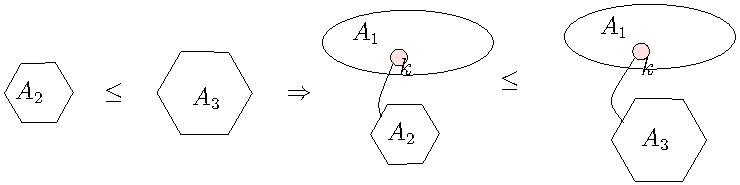
\includegraphics[scale=0.7]{Figures/Thm1intuition}
\end{center}
\proof
Let us denote by $A_{12}$ (resp. $A_{13}$) the OA resulting from $A_1\subst{A_2}{k}$ (resp. $A_1\subst{A_3}{k}$),  to prove the theorem it is sufficient to prove that there exists a relation between states of the two OA that satisfies the conditions of the Definition \ref{Def:OA-Refinement}. 

We denote $A_1=  \OA{S_1}{s_{01}}{J_1}{V_1}{\sigma_{01}}{T_1}$ and \(A_2 = \OA{S_2}{s_{02}}{J_2}{V_2}{\sigma_{02}}{T_2}\) and $A_3 = \OA{S_3}{s_{03}}{J_3}{V_3}{\sigma_{03}}{T_3}$.

% The proof requires  to rename the variables of one instance of the two $A_3$ automata to avoid clashes in variable names (this is required by the definition of refinement). In practice we will use superscripts ${}^1$ and ${}^2$ to distinguish elements of the two instances of $A_3$.

Let $R$ be the refinement relation relating states of $A_2$ and $A_3$. 
Let us denote with $t^2$ and $t^3$  the elements of $A_2$ and $A_3$ respectively.
Consider any two states $s_{12} = \mpar{s^1_1,s_2}$ and $s_{13} = \mpar{s^2_1,s_3}$ ($s^1_1$ and $s^2_1$  are the same with renaming). We define a relation $R'$ relating states of $s_{12}$ and $s_{13}$ as follows:
\[ R' \mpar{s_{12}, s_{13}} = R\mpar{s_{2}, s_{3}} \land \reach{A_{12}}(s_{12}) \wedge \bigwedge_\subbox{v_1\in V_1}
 v^1_1=v^2_1\wedge s^1_1 = s^2_1\]
Let us denote $H'=H\cup J_1 \setminus\{k\}$.
We want to prove that $\mpar{R', H'}$  is a hole-tracking simulation of $A_{12}$ and $A_{13}$. As for the previous proof we deal with cases:
\begin{enumerate}
\item \TODO{I skip it, I think the same as previous theorem}

\item Second, we need to prove for any OT $t_{12}$ in $T_{12}$ originating from $s_{12}$

\begin{align*}
		&  \OTx{12}{}{12}{12} \in \fOT{s_{12}}
\end{align*}		
there exists an indexed family $t_{13x}$ of OTs originating from $s_{13}$ that simulates it: 
\begin{align*}
		&  \mpar{\OTx{13}{x}{13x}{13x} \in \fOT{s_{13}}}^{x \in X}
\end{align*}	
such that  $\mpar{\forall x \in X, J'_{13x} \cap H' = J'_{12} \cap H'}$ and
\begin{multline*}	
V_{12} \uplus V_{13} \uplus \fvars{t_{12}} \vdash\\ R'\mpar{s_{12}, s_{13}} \wedge g_{12} \implies \operatorname*{\bigsymb{\bigvee}}_{x \in X} \mpar{\everymath{\displaystyle}\begin{array}{l}
			\alpha_{12} = \alpha_{13x} \wedge \bigwedge_\subbox{j \in J'_{13x} \cap H'} \beta_{12j} = \beta_{13xj} \wedge\\[12pt]
			 g_{13x} \wedge R'\mpar{s'_{12}, s'_{13x}}\psubst{\psi_{12} \uplus \psi_{13x}}
		\end{array}} 
	\end{multline*}
By definition of composition and OA refinement we have: 
\begin{align*}
&V_{12}= V^1_1\uplus V_3 \text{ and }
V_{13}= V^2_1\uplus V_3\\
& H'=H\uplus J_1 \setminus \{k\} \subseteq J_1\uplus \mpar{J_2 \cap J_3} \setminus \{k\}= \mpar{J^1_1\uplus J_2 \setminus \{k\} } \cap \mpar{J^2_1\uplus J_3 \setminus \{k\}} \\ &\,\,\,\,\, = J_{12 } \cap J_{13} 
\end{align*}
We have by hypothesis $\wrel{A_2}{A_3}{H}$, then for any open transition $t_2$ in $T_2$  originating from $s_2$:
\begin{align*}
\OTx{2}{}{2}{2} \in \fOT{s_2}
\end{align*}
there exists an indexed family of OTs originating from $s_{3}$: 
\begin{align*}
\mpar{\OTx{3}{x}{3x}{3x} \in \fOT{s_{3}}}^{x \in X} 
\end{align*}
such that $\forall x \in X, J'_{3x} \cap H = J'_2 \cap H$ and
\begin{multline*}
%\everymath{\displaystyle}
V_2 \uplus V_3 \uplus \fvars{t_2} \vdash\\ R\mpar{s_2, s_3} \wedge g_2 \implies \operatorname*{\bigsymb{\bigvee}}_{x \in X} \mpar{\everymath{\displaystyle}
\begin{array}{l}
			\alpha_2 = \alpha_{3x} \wedge \bigwedge_\subbox{j \in J'_{3x} \cap H} \beta_{2j} = \beta_{3xj} \nwedge\\
			 g_{3x} \wedge R\mpar{s'_2, s'_{3x}}\psubst{\psi_2 \uplus \psi_{3x}}
		\end{array}}  \qquad \quad (*)
\end{multline*}	
\smallskip



Consider any transition $t_{12}$ in $A_{12}$. Based on the definition of the composition  $t_{12}$ can be obtained from two different cases,  we will consider the two cases
separately.


\paragraph{First case: Both automata perform a transition.} The transition $t_{12}$  is obtained by the composition of transition $t_2=\OTx{2}{}{2}{2}$ and a transition \[t_1^1=
\OT{ s^1_1}{{s^1_1}'}{\alpha_1^1}{   {(\beta^1_{1j})^{j \in J^{1 \prime}_1} }}{ g^1_1 }{ \psi^1_1} \qquad \text{ when } k \in {J^1_{1}}^{\prime}
\] The result:
%%%% Attention deactiver ici
\[
t_{12} = \OT{\mpar{s^1_1, s_2}}{\mpar{{s^1_1}',s'_2 }}{\alpha^1_1}{{\beta^1_{1j}}^{j \in J^{1 \prime}_1 \setminus \{k\}} \uplus  {(\beta_{2j})^{j \in J^{\prime}_2} }}{g^1_1 \wedge g_2 \wedge \alpha^1_1 = \beta_{2k}}{\psi^1_1 \uplus \psi_2} \qquad \text{ where } k \in {J^1_{1}}^{\prime} 
\]

We then obtain a family of OTs by the simulation of $A_2$ by $A_3$ (as stated above).
By hypothesis we have $k \in H$, so in the case where $k \in {J^1_{1}}^{\prime}$, we deduce that $k \in J'_{3x}$ we can  then build  a family of OTs $t_{13x}^{x\in X}$ with the same transition, up to renaming, as the one used to build $t_{12}$ (i.e. $t_1^1$), where ${s^2_{1}}^\prime$ is the same as ${s^1_{1}}^\prime$ up to renaming.
\[
t_{13x} = \left(\OT{\mpar{s^2_1, s_3}}{\mpar{{s^2_{1}}',s'_{3x}}}{\alpha^2_{1}}  {{(\beta^2_{1j})^{j \in J^{2 \prime}_1}}\uplus \beta_{3xj}^{j \in J'_{3x}  \setminus \{k\}} }{g_{3x} \wedge g^2_1 \wedge \alpha^2_1 = \beta_{3xk}}{\psi_{3x} \uplus \psi^2_1}
\right)^{x\in X}\]
Recall that in this case  $k \in {J^1_{1}}^{\prime}$, so $\forall x \in X$ we have:
\begin{align*}
  J'_{13x} \cap H'  
&=((J'_{3x}  \setminus \mbrc{k})\uplus J^{2 \prime}_{1} ) \cap (H\uplus J_1 \setminus\{k\} )\\
&=((J'_{3x}\cap (H\uplus J_1))\uplus (J^{2 \prime}_{1}\cap (H\uplus J_1)))\setminus \mbrc{k}\\
&=((J'_{3x}\cap H)\uplus (J^{2 \prime}_{1}\cap  J_1))\setminus \mbrc{k}\text{ since } J_1\cap J'_{3x} = \emptyset \text{ and } H\cap J^{2 \prime}_{1} = \emptyset\\
& =((J'_{3x}\cap H)\uplus J^{2 \prime}_{1})\setminus \mbrc{k}\text{ since } J^{2 \prime}_{1}\subseteq J_1\\
& =((J'_2\cap H)\uplus J^{1 \prime}_{1})\setminus \mbrc{k} \text{ since } J^{1 \prime}_{1}=J^{2 \prime}_{1} \text{ and } J'_2 \cap H = J'_{3x} \cap H\\
&= ((J'_2 \cap H) \uplus (J^{1 \prime}_{1} \cap J_1)) \setminus \mbrc{k}\text{ since } J^{1 \prime}_{1}\subseteq J_1\\ 
& = (J'_2\cap (J_1 \uplus H)) \uplus ((J^{1 \prime}_{1} \cap (J_1 \uplus H)) \setminus \mbrc{k} \text{ since } J_1\cap J'_{2} = \emptyset \text{ and } H\cap J^{1 \prime}_{1} = \emptyset\\
		& = \mpar{(J'_2  \uplus J^{1 \prime}_{1})\setminus \mbrc{k}} \cap \mpar{(J_{1} \uplus H) \setminus \mbrc{k}}\\
		& = J'_{12} \cap H'
\end{align*}	

In this case the composition gives: \[g_{12} \Leftrightarrow g^1_1 \wedge g_2 \wedge \alpha^1_1=\beta_{2k} \text{ and }
g_{13x}  \Leftrightarrow g^2_1 \wedge g_{3x} \wedge  \alpha^2_1=\beta_{3xk}\]
As $k \in H$ we have   
$\alpha^1_1= \alpha^2_1$ then we  deduce:
\[g^1_1 \wedge \alpha^1_1=\beta_{2k}  \Leftrightarrow g^2_1 \wedge \alpha^2_1= \beta_{3xk}\]



The proof of the rest  is based on the following facts: 
\begin{enumerate}
\item     By construction of  $t_{12}$ and $t_{13x}$ we have $\alpha_{12}=
\alpha^1_{1}$ and $\alpha_{13x}=\alpha^2_{1}$. Since  $\alpha^1_{1}$ and  $\alpha^2_{1}$ are the same (up to renaming) we deduce: 
$\alpha_{12} = \alpha_{13x}$.
\item By composition we have also: \\ $\beta_{12j}^{j\in J'_{12}}= (\beta^1_{1j})^{j \in J^{1 \prime}_{1} \setminus \{k\}} \uplus   (\beta_{2j})^{j \in J'_{2} }$
and $\beta_{13xj}^{j\in J'_{13}}= (\beta^2_{1j})^{j \in J^{2 \prime}_{1}  \setminus \{k\}}  \uplus \beta_{3xj}^{j \in J'_{3x}  \setminus \{k\}}$\\
Therefore, we have for all $j\in J'_{12}$ (recall that $J'_{12}=J'_{13}$):  \[\beta_{12j} = \beta_{13xj} \Rightarrow (j\in J^{1\prime}_1 \land \beta^1_{1j} = \beta^2_{1j}) \vee (j\in J'_2 \land \beta_{2j}= \beta_{3xj})\]
\item 
Considering $\beta^1_{1j}$ and  $\beta^2_{1j}$  are the same (up to renaming)  we have: \\
${\displaystyle V^1_{1} \uplus V^2_{1} \uplus \fvars{t_{12}} \vdash \bigwedge_\subbox{v_1\in V_1}\!\! v^1_1=v^2_1\implies \bigwedge_\subbox{j \in J^{2 \prime}_1} \beta^1_{1j}= \beta^2_{1j}}$\\
We compose by disjunction with the following hypothesis (part of formula $(*)$).\\ $V_{2} \uplus V_{3} \uplus \fvars{t_2}  \vdash {\displaystyle \bigwedge_\subbox{j \in J'_{3x} \cap H} \beta_{2j} = \beta_{3xj}}$
\begin{align*}
 V_{2} \uplus V_{3}  \uplus V^1_{1} \uplus V^2_{1} \uplus \fvars{t_{12}}\vdash &    \bigwedge_\subbox{v_1\in V_1}\!\! v^1_1=v^2_1 \implies {\displaystyle \bigwedge_\subbox{j \in J'_{3x} \cap H} \beta_{2j} = \beta_{3xj}} \vee {\displaystyle \bigwedge_\subbox{j \in J^{2 \prime}_1} \beta^1_{1j}= \beta^2_{1j}}\\
\Rightarrow  V_{12} \uplus V_{13}  \uplus \fvars{t_{12}}\vdash & \bigwedge_\subbox{v_1\in V_1}\!\! v^1_1=v^2_1\implies {\displaystyle \bigwedge_\subbox{j \in (J'_{3x}   \cap H)\uplus J^{2 \prime}_1 } \beta_{12j} = \beta_{13xj}} \\  
\Rightarrow  V_{12} \uplus V_{13}  \uplus \fvars{t_{12}}\vdash & \bigwedge_\subbox{v_1\in V_1}\!\! v^1_1=v^2_1\implies {\displaystyle \bigwedge_\subbox{j \in    ((J'_{3x}   \cap H)\uplus J^{2 \prime}_1)\setminus \{k\} } \beta_{12j} = \beta_{13xj}} \\
\Rightarrow    V_{12} \uplus V_{12}  \uplus \fvars{t_{12}}\vdash & \bigwedge_\subbox{v_1\in V_1}\!\! v^1_1=v^2_1\implies {\displaystyle \bigwedge_\subbox{j \in (J'_{13x}   \cap H') } \beta_{12j} = \beta_{13xj}}
\end{align*}
\end{enumerate}

We can extend the valuation context of the variables to cover the variables of the transitions $t_1$ and variables $V_1^1$ and $V_1^2$ in the formula $(*)$.
By using the statements resulting from the cases (a), (b) and (c), we get:
\begin{multline*}
V_{13} \uplus V_{13}  \uplus \fvars{t_{12}} \vdash\\
R\mpar{s_2, s_{3}} \wedge \mpar{g_2 \wedge g^1_1 \wedge \alpha^1_1=\beta_{2k}}\wedge \bigwedge_\subbox{v_1\in V_1}  v^1_1=v^2_1 %\wedge s^1_1=s^2_1
\implies  \hspace{12em}\\
\operatorname*{\bigsymb{\bigvee}}_{x \in X} \mpar{\everymath{\displaystyle}
\begin{array}{l}
			\alpha_{12} = \alpha_{13x} \wedge \bigwedge_\subbox{j \in (J'_{13x} \cap H')} \beta_{12j}\! =\! \beta_{13xj}\nwedge\\
			  g_{3x} \wedge R\mpar{s'_2, s'_{3x}}\psubst{\psi_2 \uplus \psi_{3x}}
		\end{array}}  \wedge g^2_1 \wedge \alpha^2_1=\beta_{3xk} 
%\wedge \bigwedge_\subbox{v_3\in V_3}  v^1_3=v^2_3\wedge s^1_3=s^2_3
\end{multline*}	
That can be re-written as follows:
\begin{multline*}
V_{12} \uplus V_{13} \uplus \fvars{t_{12}}  \vdash\\
R\mpar{s_2, s_{3}} \wedge g_{12}  \land \bigwedge_\subbox{v_1\in V_1} v^1_1=v^2_1
\implies  \operatorname*{\bigsymb{\bigvee}}_{x \in X} \mpar{\everymath{\displaystyle}
\begin{array}{l}
			\alpha_{12} = \alpha_{13x} \wedge \bigwedge_\subbox{j \in J'_{13x} \cap H'} \beta_{12j} = \beta_{13xj} \nwedge\\
			g_{13x} \wedge R\mpar{s'_2, s'_{3x}}\psubst{\psi_2 \uplus \psi_{3x}}
		\end{array}}   
\end{multline*}	


Moreover, we have  for any transition $t_1 $ in $A_1$ relating $s^1_1$ and ${s^1_1}^{\prime}$ the following:
\begin{multline*}
V_{12} \uplus V_{13}  \uplus \fvars{t_{12}} \vdash\\
\bigwedge_\subbox{v_1\in V_1}\!\! v^1_1=v^2_1  \wedge s^1_1 = s^2_1 \implies \bigwedge_\subbox{v_1\in V_1}\!\! \psi_{12}(v^1_1)=\psi_{13x}(v^2_1)  \wedge s^{1\prime}_1 = s^{2\prime}_1 
\end{multline*}

From the two previous formula, we get: 
\begin{multline*}
V_{12} \uplus V_{13}  \uplus \fvars{t_{12}} \vdash\\
R\mpar{s_2, s_{3}} \wedge g_{12}  \land \bigwedge_\subbox{v_1\in V_1} v^1_1=v^2_1  \wedge s^1_1 = s^2_1 
\implies \hspace{12em}\\ \operatorname*{\bigsymb{\bigvee}}_{x \in X} \mpar{\everymath{\displaystyle}
\begin{array}{l}
			\alpha_{12} = \alpha_{13x} \wedge \bigwedge_\subbox{j \in J'_{13x} \cap H'} \beta_{12j} = \beta_{13xj} \nwedge g_{13x} \wedge \\
			 R\mpar{s'_2, s'_{3x}}\psubst{\psi_2 \uplus \psi_{3x}} \wedge \bigwedge_\subbox{v_1\in V_1}\!\! \psi_{12}(v^1_1)=\psi_{13x}(v^2_1)  \wedge s^{1\prime}_1 = s^{2\prime}_1
		\end{array}}   
\end{multline*}	


 Furthermore, according to the Definition \ref{Def:Reach} (reachability, applied to the composed automaton \(A_1\subst{A_2}{k}\)) we have, for all $t_{12} \in T_{12}$:
\[ \fvars{t_{12}} \vdash \left(\reach{A_{12}}\mpar{s_{12}} \wedge g_{12} \implies \reach{A_{12}}\mpar{s_{12}'}\psubst{\psi_{12}}\right) \]	

Thus, we get:
\begin{multline*}
V_{12} \uplus V_{13}  \uplus \fvars{t_{12}} \vdash\\
R\mpar{s_2, s_{3}} \wedge g_{12} \land \reach{A_{12}}\mpar{s_{12}} \land \bigwedge_\subbox{v_1\in V_1} v^1_1=v^2_1  \wedge s^1_1 = s^2_1 
\implies \hspace{12em}\\ \operatorname*{\bigsymb{\bigvee}}_{x \in X} \mpar{\everymath{\displaystyle}
\begin{array}{l}
			\alpha_{12} = \alpha_{13x} \wedge \bigwedge_\subbox{j \in J'_{13x} \cap H'} \beta_{12j} = \beta_{13xj} \nwedge g_{13x} \wedge \\
			 R\mpar{s'_2, s'_{3x}}\psubst{\psi_2 \uplus \psi_{3x}} \land \reach{A_{12}}\mpar{s_{12}'}\psubst{\psi_{12}} \\
\wedge \bigwedge_\subbox{v_1\in V_1}\!\! \psi_{12}(v^1_1)=\psi_{13x}(v^2_1)  \wedge s^{1\prime}_1 = s^{2\prime}_1
		\end{array}}   
\end{multline*}	



Because of the independence of the substitution domains, we simplify and get the expected formula:
\begin{multline*}
V_{12} \uplus V_{13}  \uplus \fvars{t_{12}} \vdash
R'\mpar{s_{12}, s_{13}} \wedge g_{12} 
\implies \hspace{10em}\\ \operatorname*{\bigsymb{\bigvee}}_{x \in X} \mpar{\everymath{\displaystyle}
\begin{array}{l}
			\alpha_{12} = \alpha_{13x} \wedge \bigwedge_\subbox{j \in J'_{13x} \cap H'} \beta_{12j} = \beta_{13xj} \nwedge g_{13x} \wedge 
			 R'\mpar{s'_{12}, s'_{13x}}\psubst{\psi_{12} \uplus \psi_{13x}}
		\end{array}}   
\end{multline*}	

\paragraph{Second case: Only the encompassing automaton performs a transition.}
  $t_{12}$ is obtained by the transition 
$t^1_1=\OT{ s^1_1}{{s^1_1}'}{\alpha_1^1}{{(\beta^1_{1j})^{j \in J^{1 \prime}_1} }}{ g^1_1 }{ \psi^1_1}$  alone with the state $s_2$ unchanged, if $k \not\in {J^1_{1}}^{\prime}$
\[t_{12} = \OT{\mpar{s^1_1, s_2}}{\mpar{{s^1_1}', s_2}}{\alpha_1^1}{ {(\beta^1_{1j})^{j \in J^{1 \prime}_1} }}{g^1_1}{\psi^1_1}
\]
%As stated above, from the simulation of $A_2$ by $A_3$ we get a  family of OTs $t_{3x}^{x\in X}$. The composition of this family of OTs 
% with the same transitions of $A_1$ (up to renaming) as those used to build $t_{12}$ 
%produces  a family of OTs $t_{13x}^{x\in X}$ in the form:
%\[t_{13x} = \left(\OT{\mpar{s^2_1, s_{3}}}  {\mpar{s^{2\prime}_1, s_{3}}}  {\alpha_1^2}{{(\beta^2_{1j})^{j \in J^{2 \prime}_1} }}{ g^2_1 }{\psi^2_1} \right) \]
 
\TODO{NEW -- a refaire en plus joli}

The hole is not involved we can define $t_{13}$ with the same transition $t_1$ of $A_1$ (where elements of $t_1$ are the same as above modulo renaming of variables):
\[t_{13} = \OT{\mpar{s^1_1, s_3}}{\mpar{{s^2_1}', s_3}}{\alpha_1^2}{ {(\beta^2_{1j})^{j \in {J^{2}_1}'} }}{g^2_1}{\psi^2_1}
\]
We thus take $({t_{13 x}})^{x\in X} = \{t_{13}\}$.
$\forall x \in X$ we have $J'_{13x} =  {J^{2}_1}'$ and trivially:
\begin{align*}		
J'_{13x} \cap H' & =  J^{2 \prime}_1 \cap \mpar{J_1 \uplus H \setminus \mbrc{k}} \\
& =  J^{1 \prime}_1 \cap \mpar{J_1 \uplus H \setminus \mbrc{k}} \text{ since }  J^{2 \prime}_1 =  J^{1 \prime}_1\\
& = \mpar{J'_{12}\cap H' }
\end{align*}



Moreover, we have by definition 
\[R' \mpar{s_{12}, s_{13}} =  R\mpar{s_{2}, s_{3}} \land \reach{A_{12}}(s_{12}) \wedge \bigwedge_\subbox{v_1\in V_1} v^1_1=v^2_1\wedge s^1_1 = s^2_1 \]
Thus, because transitions $t^1_1$ and  $t^2_1$ are the same:
\[R' \mpar{s_{12}, s_{13}} \implies
\underbrace{R\mpar{s_{2}, s_{3}} \land \reach{A_{12}}(s_{12}) \wedge \bigwedge_\subbox{v_1\in V_1} v^1_1=v^2_1\wedge {s^1_1}^\prime = {s^2_1}^\prime}_{R' \mpar{s'_{12}, s'_{13}}}
\]


Moreover, we have  the following:
\begin{multline*}
V_{12} \uplus V_{13}  \uplus \fvars{t_{12}} \vdash\\
\bigwedge_\subbox{v_1\in V_1}\!\! v^1_1=v^2_1  \wedge s^1_1 = s^2_1 \implies \bigwedge_\subbox{v_1\in V_1}\!\! \psi_{12}(v^1_1)=\psi_{13}(v^2_1)  \wedge s^{1\prime}_1 = s^{2\prime}_1 
\end{multline*}
  

 
 Furthermore, according to the Definition \ref{Def:Reach} (reachability, applied to the composed automaton \(A_1\)) we have, for all $t_{12} \in T_{12}$:
\[ \fvars{t_{12}} \vdash \left(\reach{A_{12}}\mpar{s_{12}} \wedge g_{12} \implies \reach{A_{12}}\mpar{s_{12}'}\psubst{\psi_{12}}\right) \]	

Because $\alpha_{12}$ and $\alpha_{13}$ are the same, and also  $\beta_{12}$ and $\beta_{13}$ are the same (modulo renaming of variables), we deduce from the above the expected formula (instantiated with $X$ a singleton): %From the above we can deduce the expected formula:
\begin{multline*}
V_{12} \uplus V_{13}  \uplus \fvars{t_{12}} \vdash
R'\mpar{s_{12}, s_{13}} \wedge g_{12} 
\implies \hspace{10em}\\ %\operatorname*{\bigsymb{\bigvee}}_{x \in X}
 \mpar{\everymath{\displaystyle}
%\begin{array}{l}
			\alpha_{12} = \alpha_{13} \wedge \bigwedge_\subbox{j \in J'_{13} \cap H'} \beta_{12j} = \beta_{13j} \nwedge g_{13} \wedge 
			 R'\mpar{s'_{12}, s'_{13}}\psubst{\psi_{12} \uplus \psi_{13}}
%		\end{array}
}   
\end{multline*}	



%By hypothesis we have   $k \in H$ and $k \not\in J^{1\prime}_1$, then $k \not\in J^{2\prime}_1$.    



\item Lastly, we have to prove the satisfaction of the deadlock reduction condition, i.e., for all $\mpar{s_{12}, s_{13}} \in S_{12} \times S_{13}$
\begin{multline*}
V_{12} \uplus V_{13}  \vdash  R'\mpar{s_{12}, s_{13}} \nwedge  \neg(\bigvee_\subbox{t_{12} \in \fOT{s_{12}}} \fguard{t_{12}}) \implies   \neg (\bigvee_\subbox{t_{13} \in \fOT{s_{13}}} \fguard{t_{13}}) 
\end{multline*}

Let's start  with the hypothesis of the theorem stating that $\wrel{A_2}{A_3}{H}$, thus we have for all  $\mpar{s_2, s_3} \in S_2 \times S_3$ 
\begin{multline*}
V_2 \uplus V_3  \vdash R\mpar{s_2, s_3} \nwedge \neg (\bigvee_\subbox{t_2 \in \fOT{s_2}} \fguard{t_2}) \implies   \neg(\bigvee_\subbox{t_3 \in \fOT{s_3}} \fguard{t_3})
\end{multline*}

By hypothesis  the composition  \(A_1\subst{A_2}{k}\) is non-blocking,  then according to the Definition \ref{Def:Non-block} we have for all state $s_{12}$: 


\begin{multline*}
V_{12} \uplus \biguplus_\subbox{t_1 \in \fOT{s_1}} \fvars{t_1}  \vdash  \left(\reach{A_{12}(s_{12})} \land \bigvee_\subbox{t_1 \in \fOT{s_1}} \fguard{t_1}\right) \implies \bigvee_\subbox{t_{12} \in \fOT{s_{12}}} \fguard{t_{12}}
\end{multline*}

Which implies 
\begin{multline*}
V_{12} \uplus \biguplus_\subbox{t_1 \in \fOT{s_1}} \fvars{t_1}  \vdash 
\neg{ \bigvee_\subbox{t_{12} \in \fOT{s_{12}}} \fguard{t_{12}}}
\implies 
\left(\neg{\reach{A_{12}(s_{12})} }\lor \neg{\bigvee_\subbox{t_1 \in \fOT{s_1}} \fguard{t_1}}
\right)
\end{multline*}

Additionally, each transition $t_{13}$ of OT$(s_{13})$ is of the form $
g_1\land g_3 \land g$ with $g_1$ a guard of a transition $t_{1}$ of OT$(s_{1})$.
Thus 
\[
\neg{\bigvee_\subbox{t_1 \in \fOT{s_1}} \fguard{t_1}}  \implies \neg (\bigvee_\subbox{t_{13} \in \fOT{s_{13}}} \fguard{t_{13}}) \]

Thus we have, as $R$ contains the reachability of state $s_{12}$:\TODO{faire une jolie equation}
\begin{multline*}
V_{12} \uplus V_{13}  \vdash  R'\mpar{s_{12}, s_{13}} \nwedge  \neg(\bigvee_\subbox{t_{12} \in \fOT{s_{12}}} \fguard{t_{12}}) \\
\implies \reach{A_{12}(s_{12})} \land \left(\neg{\reach{A_{12}(s_{12})} }\lor
\neg (\bigvee_\subbox{t_{13} \in \fOT{s_{13}}} \fguard{t_{13}})\right) \\
\implies
\neg (\bigvee_\subbox{t_{13} \in \fOT{s_{13}}} \fguard{t_{13}})
\end{multline*}
\qed

\end{enumerate}






\end{document}
